% ══════════════════════════════════════════════════════════════════════════════
%  CHAPTER 7: COSMIC MICROWAVE BACKGROUND
% ══════════════════════════════════════════════════════════════════════════════

\chapter{Cosmic Microwave Background (CMB) (Lecture 15-19)}
% =══════════════════════════════════════════════════════════════════════════════
\section{Recombination and photon decoupling}
% -──────────────────────────────────────────────────────────────────────────────
\subsection{Recombination}
\begin{intuition}
    Recombination is the process where free electrons and protons combine to form neutral hydrogen atoms. 
    \[
        p + e^- \leftrightarrow H + \gamma
    \]
    This occurs when the universe cools down to about $T\sim 3000$ K, which corresponds to a redshift of $z\sim 1100$. \\
    
    Before recombination, the universe is a hot plasma that is opaque to photons due to Thomson scattering. After recombination, the universe becomes transparent, allowing photons to travel freely. This is the epoch when the CMB photons were last scattered, and hence we can observe them today as a snapshot of the universe at that time.
\end{intuition}

\bigskip \noindent
\begin{foundation}
    Recall, the number density of particles i in non-relativistic thermal equilibrium is given by:
    \[
        n_i = g_i \left( \frac{m_i T}{2\pi} \right)^{3/2} e^{-(m_i - \mu_i)/T}
    \]
    Using $m_p \approx m_H$ and $\mu_p + \mu_e = \mu_H$ (as $\mu_\gamma = 0$), we can get the number density of H atoms:
    \small \begin{align*}
        n_H &= g_H \left( \frac{m_H T}{2\pi} \right)^{3/2} e^{-(m_H - \mu_H)/T} \\
        &= g_H \left( \frac{m_p T}{2\pi} \right)^{3/2} e^{-(m_p + m_e - B - \mu_p - \mu_e)/T} \\
        &= \frac{g_H}{g_p g_e} \left( g_p \left( \frac{m_p T}{2\pi} \right)^{3/2} e^{-(m_p - \mu_p)/T} \right) \left( g_e \left( \frac{m_e T}{2\pi} \right)^{3/2} e^{-(m_e - \mu_e)/T} \right)  \frac{2\pi}{m_e T}^{3/2} e^{B/T} \\
        &= \frac{g_H}{g_p g_e} n_p n_e \left( \frac{2\pi}{m_e T} \right)^{3/2} e^{B/T}
    \end{align*}
    \normalsize where $B = m_p + m_e - m_H \approx 13.6$ eV is the binding energy of hydrogen.\\

    For a H atom, it is combined by the nucleus (with spin 1/2) and the electron (with spin 1/2), thus it has a total degeneracy spin state as:
    \[
        g_H = g_p + g_e = 2 + 2 = 4
    \] \\

    Defining the ionization fraction for hydrogen only plasma as:
    \[
        Y_p = \frac{n_p}{n_B} 
    \]
    and using the above results of $g_H$, and approximation $n_H = n_B - n_p = (1 - Y_p) n_B$, we can rewrite it as:
    \begin{align*}
        (1 - Y_p) n_B &= \frac{4}{2 \times 2} n_p n_e \left( \frac{2\pi}{m_e T} \right)^{3/2} e^{B/T} \\
        (1 - Y_p) n_B &= n_p n_e \left( \frac{2\pi}{m_e T} \right)^{3/2} e^{B/T} 
    \end{align*} 
    Note using the charge neutrality condition $n_p = n_e$, and the baryon-to-photon ratio $\eta = n_B/n_\gamma$, we can simplify the equation as:
    \begin{align*}
       (1 - Y_p) n_B &= (Y_p n_B) (Y_p n_B) \left( \frac{2\pi}{m_e T} \right)^{3/2} e^{B/T} \\
       \frac{1 - Y_p}{Y_p^2} &= \eta \n_\gamma \left( \frac{2\pi}{m_e T} \right)^{3/2} e^{B/T}
    \end{align*}
    Further, using the photon number density for a blackbody radiation $n_\gamma = 2 \zeta(3) T^3/\pi^2$, we can get the Saha equation for recombination:
    \begin{align*}
        \frac{1 - Y_p}{Y_p^2} &= \eta \frac{2 \zeta(3)}{\pi^2} T^3 \left( \frac{2\pi}{m_e T} \right)^{3/2} e^{B/T} \\
        &= \eta \frac{2^{5/2} \zeta(3)}{\pi^{1/2}} \left( \frac{T}{m_e} \right)^{3/2} e^{B/T}
    \end{align*}
\end{foundation}

\bigskip \noindent
\begin{theory}
    Under the assumption of chemical equilibrium of the recombination process, we get:
    \[
        n_H = \frac{g_H}{g_p g_e} n_p n_e \left( \frac{2\pi}{m_e T} \right)^{3/2} e^{B/T}
    \]
    And hence the \textbf{Saha equation} for ionization fraction of hydrogen is:
    \[
        \frac{1 - Y_p}{Y_p^2} = \eta \frac{2^{5/2} \zeta(3)}{\pi^{1/2}} \left( \frac{T}{m_e} \right)^{3/2} e^{B/T}
    \]
\end{theory}

\bigskip \noindent
\begin{intuition}
    From the above equations, we know that when $B \ll T$, the RHS $ \ll 1$, thus $Y_p \approx 1$, which means almost all the hydrogen is ionized (i.e. all protons and electrons are free). \\

    When temperature drops to $T \ll B$, the ratio of $Y_p$ finally starts to drop. Notice that as $\eta \sim 10^{-9}$ is very small, there are very many photons per baryon, so even when $E > B$, there are still enough photons with energy greater than $B$ to ionize the hydrogen atoms, until $E \ll B$ (around $T \sim 0.3$ eV $\ll 13.6$ eV). 
\end{intuition}

\bigskip \noindent
\begin{figure}[!htbp]
    \centering
    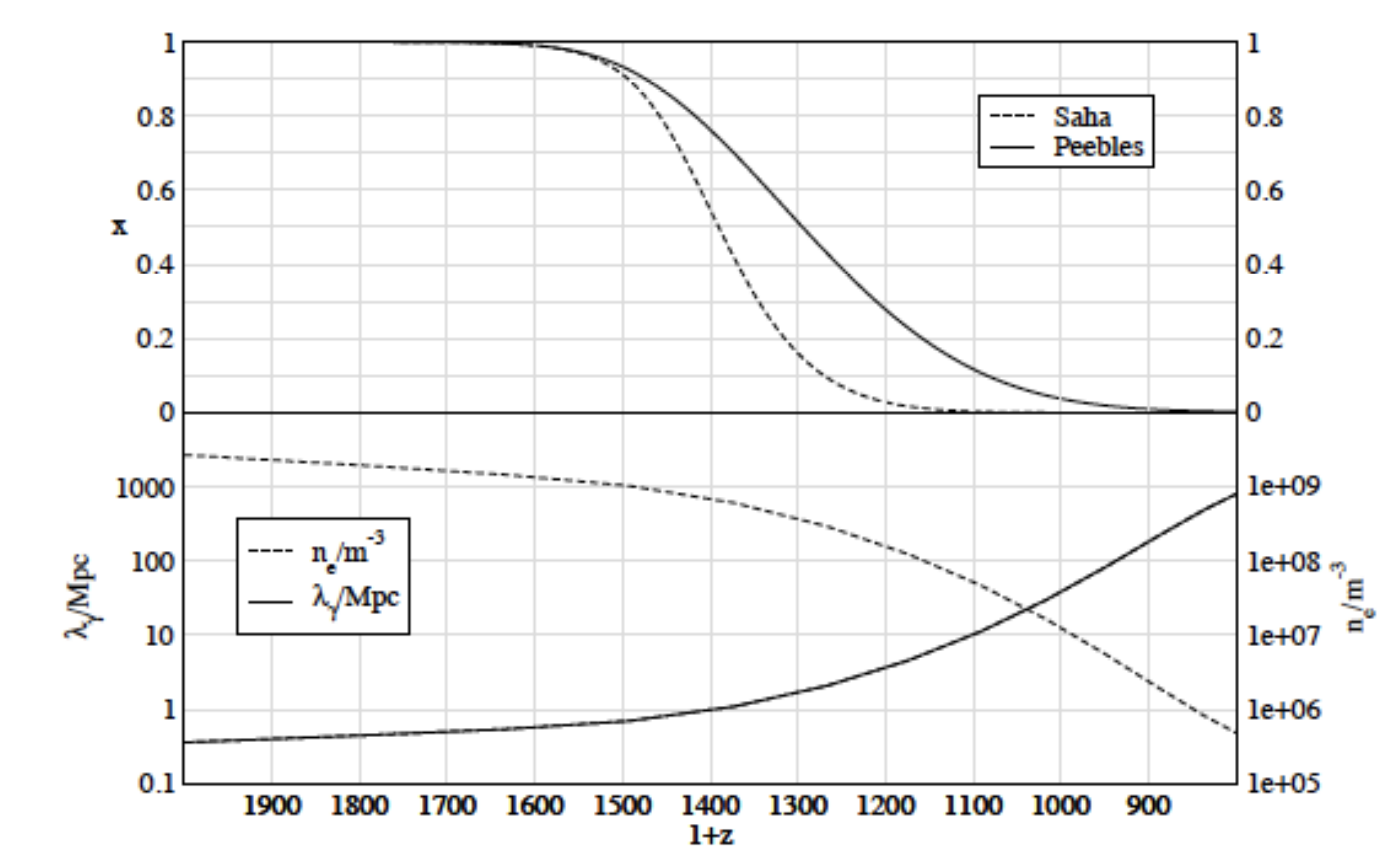
\includegraphics[width=0.8\textwidth]{images/saha_equation.png}
    \caption{The ionization fraction of hydrogen $x$ (upper) and the exact value of $n_e \& \lambda_\gamma$ (lower) as a function of redshift $z$.}
    \label{fig:saha_equation}
\end{figure}

\begin{intuition}
    From the above figure, the upper panel show the ionization fraction, the dashed curve represents the Saha equation, which calculate assuming universe is in \textbf{perfect chemical equilibrium}, while the solid curve represent the Peebles equation, which more accurate as accounting for the fact that the universe is expanding rapidly and faster than the atoms can recombine, thus the chemical equilibrium is \textbf{not perfectly} maintained, and the recombination process is "lagging behind". Hence, the Peebles equation gives a more gentle drop of the ionization fraction, and a slightly later recombination time. \\
    
    \pagebreak
    In the lower panel, the dotted curve represents the number density of free electrons $n_e$, which as the universe expands and recombines, the number density of free electrons drops significantly (from $1e+09$ to $1e+06$); At the same time, the mean free path of photons $\lambda_\gamma$ increases dramatically (from 1 Mpc to 1000 Mpc), which means the universe becomes transparent to photons, and the CMB photons can travel freely without being scattered by free electrons.
\end{intuition}

\bigskip \noindent
\begin{theory}
    Let us define the recombination $T_{rec}$ as the temperature when the ionization fraction drops to $Y_p = 0.5$, which means half of the hydrogen is ionized and half is neutral. \\
    
    Note that by Wien's law, temperature is inversely proportional to the wavelength, and hence inversely proportional to scale factor, thus we can also define the recombination redshift $z_{rec}$ as:
    \[
        1 + z_{rec} = \frac{a_0}{a_{rec}} = \frac{T_{rec}}{T_0}
    \]

    From the above figure, we can find that:
    \[
        z_{rec} \approx 1300, \quad T_{rec} \approx 0.3 \text{ eV}
    \]
\end{theory}


% -──────────────────────────────────────────────────────────────────────────────
\bigskip \noindent \bigskip \noindent \bigskip \noindent
\subsection{Photon Decoupling and CMB}
\begin{intuition}
    Although the recombination process starts at $z \sim 1300$, the universe is still not completely transparent to photons, as there are still some free electrons that can scatter photons. The photon decoupling occurs when the mean free path of photons $\lambda_\gamma$ becomes larger than the Hubble radius $H^{-1}$, which in other words, the characteristic interaction become comparable to the expansion rate of the universe $\Gamma_\gamma \sim H$ (\textbf{see chapter 5.6.5}). \\

    Thus, the decoupling temperature occurred at $Y_p \sim 0.1$, which is around:
    \[
        T_{dec} \approx 0.26 \text{ eV}, \quad z_{dec} \approx 1100
    \]
    so we can say after the photon decoupling, the "first light" in the universe is emitted at around $z \sim 1100$ with a temperature of $T \sim 3000$ K, and as it no longer interacts with matter, it can travel through the spacetime and reach us today. \\
    
    However, due to the expansion of the universe, the wavelength of the photons is stretched, and hence the temperature of the light ray is much lower than the original temperature at the time of decoupling, which is now redshifted to the microwave band, which is what we call the Cosmic Microwave Background (CMB) radiation. \\
\end{intuition}

\bigskip \noindent
\begin{theory}
    We can use the relationship between the redshift and temperature to calculate the CMB temperature today. Let $T_{dec} = 0.26 \text{ eV } = 3000$ K and $z_{dec} = 1100$, we can get:
    \[
        T_{CMB} = \frac{T_{dec}}{1 + z_{dec}} \approx 2.727 \text{ K}
    \]
\end{theory}

\bigskip \noindent
\begin{figure}[!htbp]
    \centering
    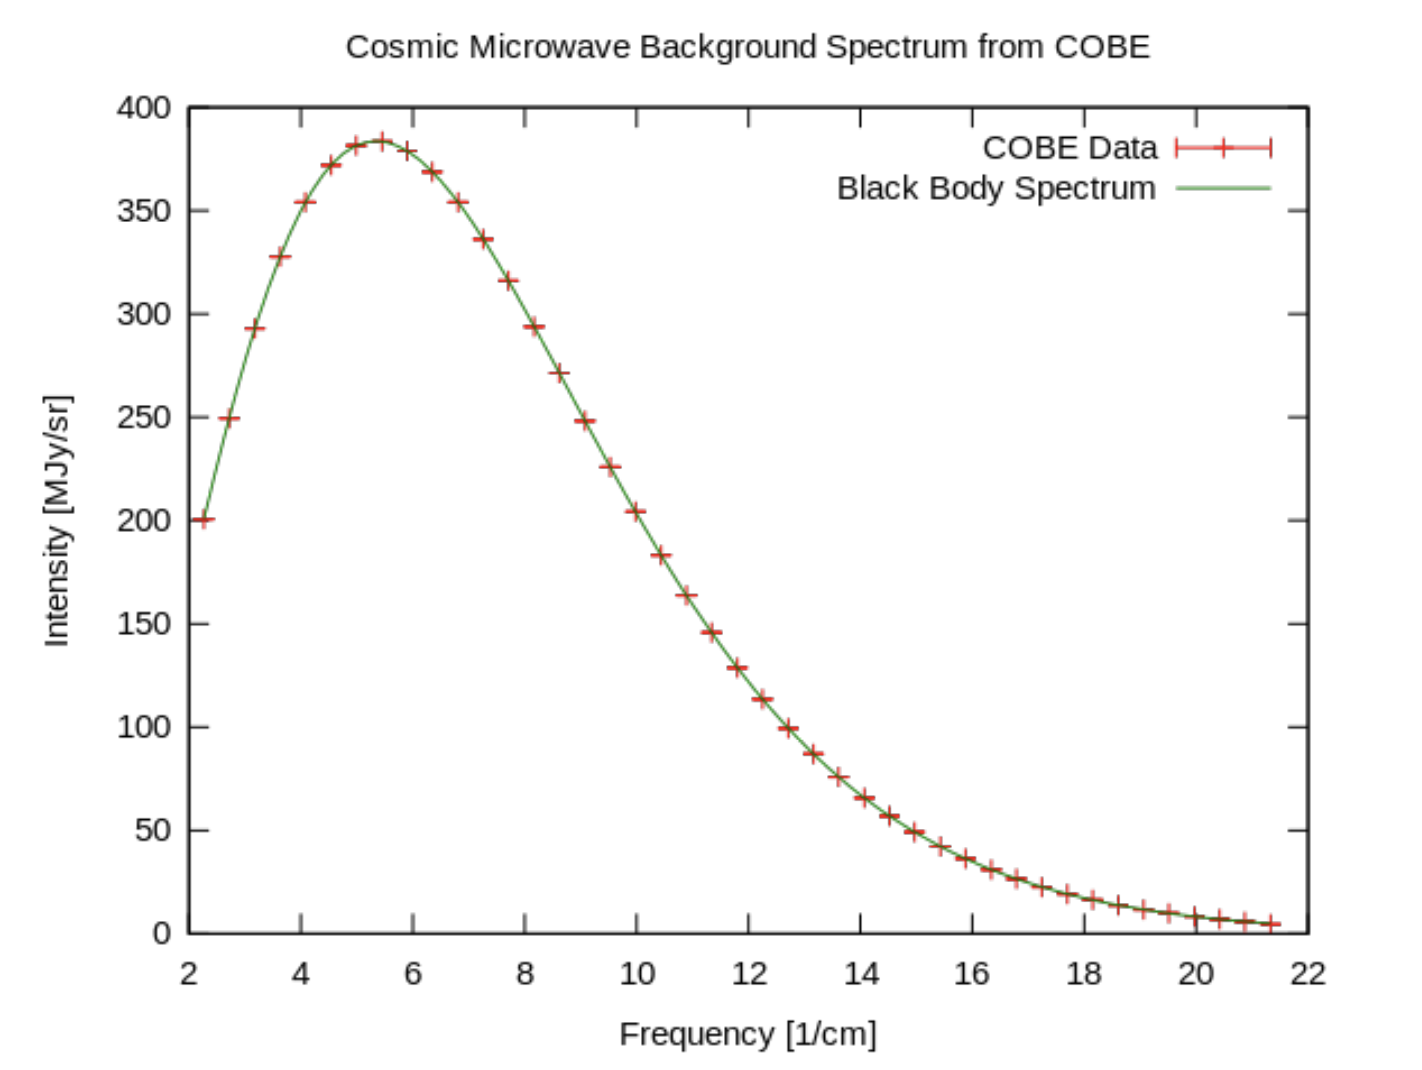
\includegraphics[width=0.8\textwidth]{images/CMB_frequency_spectrum.png}
    \caption{The CMB frequency spectrum measured by the COBE satellite with FIRAS instruments.}
    \label{fig:CMB_frequency_spectrum}
\end{figure}

\clearpage
\begin{extra}
    From the figure, the red crosses (COBE data) shows the actual measurement taken by FIRAS instruments on the COBE satellite, the tiny bars represent the incredibly small error margins; Meanwhile, the green curve represent the theoretical curve calculated by the Planck blackbody radiation formula for perfect blackbody radiation, which is given by:
    \[
        I_\nu = \frac{2 h \nu^3}{c^2} \frac{1}{e^{h\nu/k_B T} - 1}
    \]
    where $I_\nu$ is the intensity of radiation at frequency $\nu$, $h$ is the Planck constant, $c$ is the speed of light, $k_B$ is the Boltzmann constant, and $T$ is the temperature of the blackbody. \\

    We can see that red crosses perfectly match the green curve, which means the CMB radiation is an almost perfect blackbody radiation, and the temperature of the CMB can be determined by fitting the data to the Planck formula, which gives $T \approx 2.725 \pm 0.002$ K with $95\%$ confidence level. \\

    In fact, the result was so significant that it led to John Mather and George Smoot being awarded the Nobel Prize in Physics in 2006 for their work on the COBE satellite and the measurement of the CMB spectrum.
\end{extra}


\bigskip \noindent
\begin{remark}
    The CMB is a snapshot of the universe at the time of photon decoupling, which occurred about 380,000 years after the Big Bang. In fact, it is the oldest light we can observe, and hence is the earliest direct evidence we can "observed".
\end{remark}

\bigskip \noindent
\begin{extra}
    The CMB was first predicted by Ralph Alpher and Robert Herman in 1948, as a consequence of the Big Bang theory. Later, it was accidentally discovered by Arno Penzias and Robert Wilson in 1965, who were awarded the Nobel Prize in Physics in 1978 for their discovery. The CMB is a crucial piece of evidence for the Big Bang theory, and has been extensively studied by various experiments, such as COBE, WMAP, and Planck satellites.
\end{extra}

% -──────────────────────────────────────────────────────────────────────────────
%\bigskip \noindent \bigskip \noindent \bigskip \noindent
\clearpage
\subsection{Dark Ages and Reionization}
\begin{intuition}
    After photon decoupling, the universe becomes transparent to photons, and is still hot ($T\sim 3000$ K), hence showing a uniform red glow colour. After that, the universe become cooler and darker, and the photons are redshifted towards to infrared and microwave bands. As a results, the universe enters a ``dark age'' as nearly no visible light is emitted. \\

    The dark age last several hundred million years until the first stars and galaxies form ($z \sim 10$), which emit UV photons that reionize the intergalactic medium. This process is called \textbf{reionization}. Note that in this stage the gas cloud already has a very low density, thus the universe remains transparent to photons, and the CMB photons can still reach us without being scattered by the gas. \\
\end{intuition}

\bigskip \noindent
\begin{remark}
    In fact, there is no direct observation of the dark ages currently, astrophysicists are still trying different methods to probe this era, for example, using 21-cm line observations, which can trace the neutral hydrogen gas before reionization. Overall, the dark ages still remains a large observational gap in our understanding of cosmic history.
\end{remark}


% =══════════════════════════════════════════════════════════════════════════════
%\clearpage
\bigskip \noindent \bigskip \noindent \bigskip \noindent
\section{CMB anisotropies}
% -──────────────────────────────────────────────────────────────────────────────
%\subsection{Introduction of anisotropies}
\begin{figure}[!htbp]
    \centering
    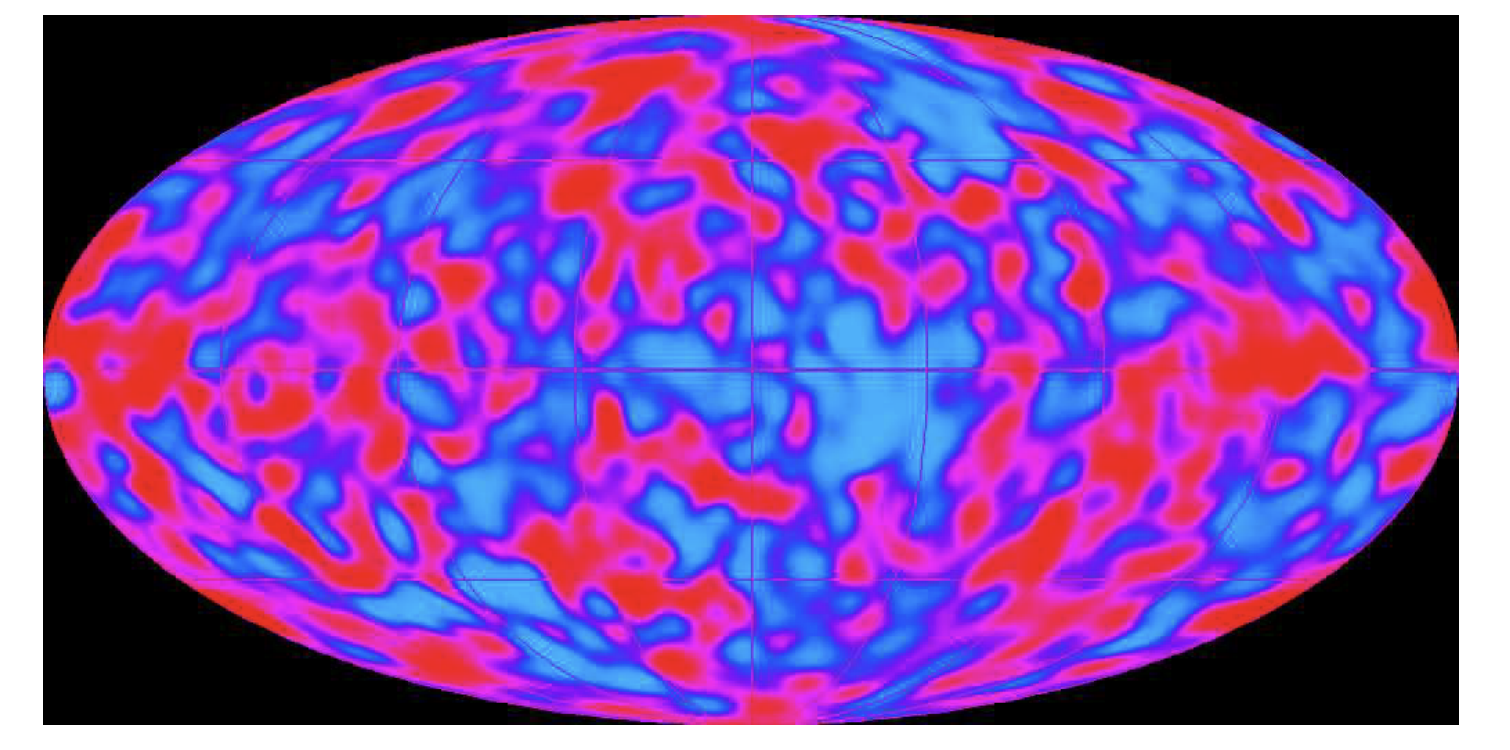
\includegraphics[width=0.7\textwidth]{images/CMB_anisotropies.png}
    \caption{The CMB anisotropies measured by the Planck satellite.}
    \label{fig:CMB_anisotropies}
\end{figure}

\begin{intuition}
    When the COBE satellite first returned the data of the CMB, Scientists found out that there are tiny fluctuations in the temperature of the CMB across the sky, which is called \textbf{CMB anisotropies}. These anisotropies are on the order of $10^{-5}$ K, which means the temperature of the CMB is not perfectly uniform, but has tiny variations. \\

    The anisotropies provide crucial information about the early universe, as they are the seeds of the large scale structure we see today. The tiny fluctuations in the CMB temperature correspond to the density fluctuations in the early universe, which eventually grow into galaxies and clusters of galaxies due to gravitational instability.
\end{intuition}

\bigskip \noindent
\begin{theory}
    Define the temperature fluctuation of any point $(\theta, \phi)$ on the sky as:
    \[
        \frac{\Delta T (\theta, \phi) }{T_0} = \frac{T(\theta, \phi) - T_0}{T_0} \sim 10^{-5}
    \]
    where $T_0$ is the average temperature of the CMB:
    \[
        T_0 = \frac{1}{4\pi} \int T(\theta, \phi) d\Omega \approx 2.725 \text{ K}
    \]
    with $d\Omega = \sin \theta d\theta d\phi$ is the solid angle element. \\
\end{theory}


\bigskip \noindent
\begin{figure}[!htbp]
    \centering
    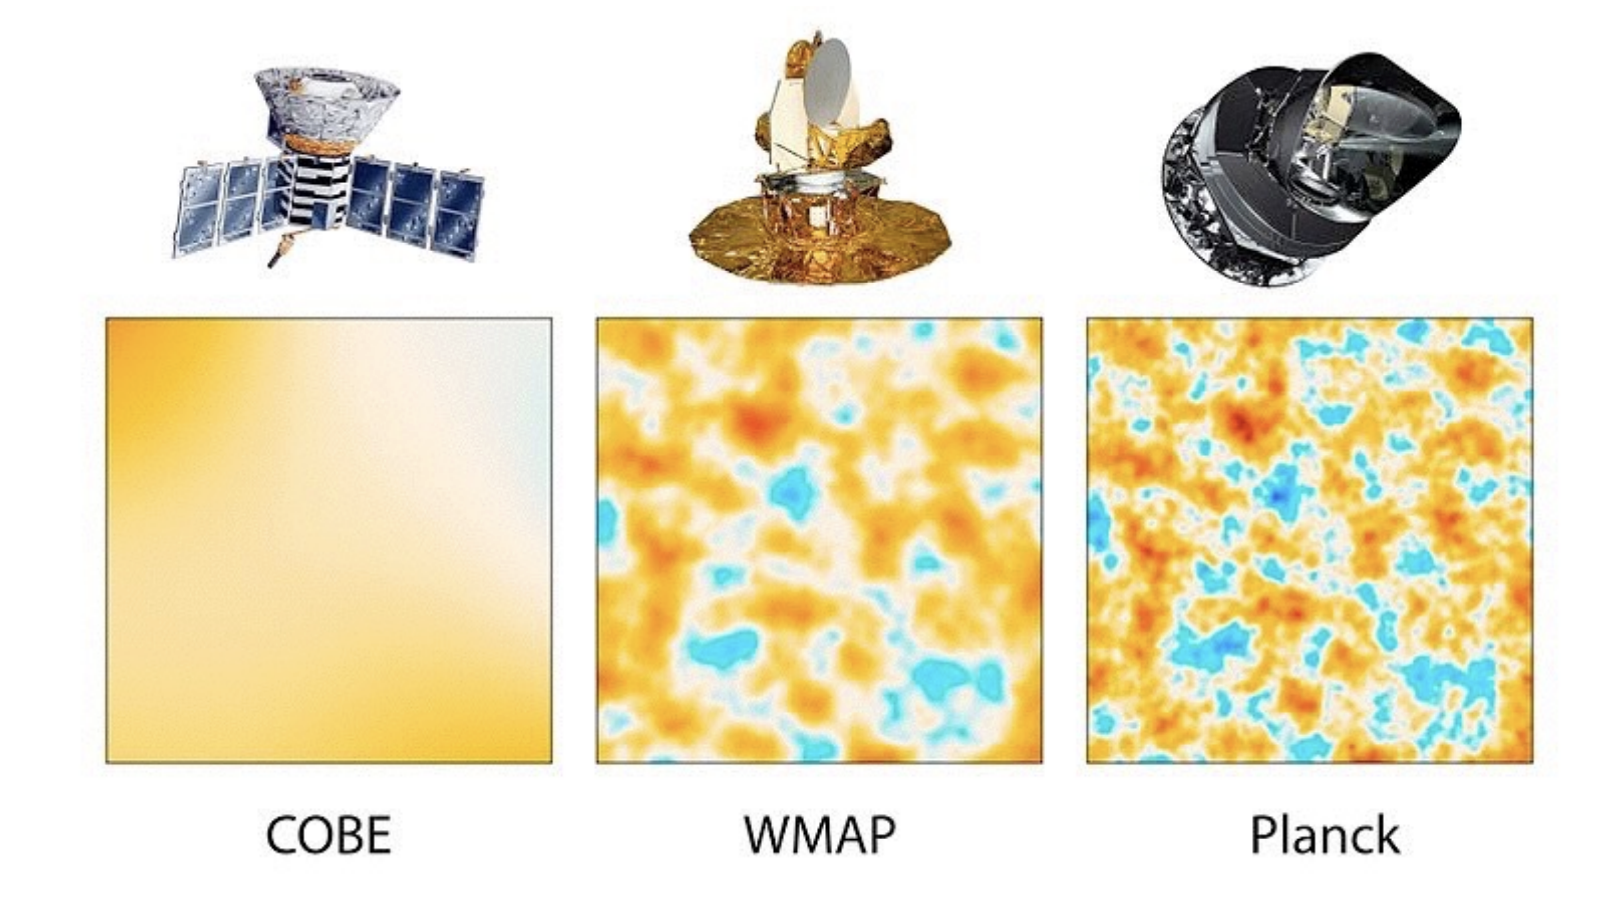
\includegraphics[width=0.8\textwidth]{images/CMB_comparison.png}
    \caption{The CMB anisotropies measured by the COBE, WMAP and Planck satellites.}
    \label{fig:CMB_comparison}
\end{figure}

\begin{extra}
    The anisotropies were first detected by the COBE satellite in 1992, however, as the angular resolution of COBE was quite low (about 7 degrees), it could only detect the anisotropies on scales larger than that. \\

    To get a higher resolution map of the CMB anisotropies, NASA launched the WMAP satellite in 2001, which had an angular resolution of about 13 arcminutes, and hence could detect the anisotropies on smaller scales. The WMAP data provided a much more detailed map of the CMB anisotropies, and allowed scientists to measure the cosmological parameters with much higher precision. \\

    After that, the Planck satellite was launched in 2009, which had an even higher angular resolution of about 5 arcminutes, and hence could detect the anisotropies on even smaller scales. The Planck data provided the most detailed map of the CMB anisotropies to date, and allowed scientists to measure the cosmological parameters with unprecedented precision. \\
\end{extra}

% -──────────────────────────────────────────────────────────────────────────────
\bigskip \noindent \bigskip \noindent \bigskip \noindent
\subsection{Spherical Harmonic Decomposition}
\begin{intuition}
    Recall Fourier decomposition, when we want to analyze a function $y = f(x)$ defined on a line, we can decompose it into a sum of sine and cosine functions with different frequencies, which is called Fourier decomposition. \\

    In the case of CMB anisotropies, we can use a similar method to decompose the temperature fluctuations on the sky, but this time is defined on a sphere, thus we need to use spherical harmonics instead of sine and cosine functions. 
\end{intuition}

\begin{foundation}
    Just like Fourier decomposition, we can approximate the CMB by a sum of periodic functions, which in this case are the spherical harmonics $Y_{lm}(\theta, \phi)$, where $l$ is the degree of the spherical harmonic, and $m$ is the order of the spherical harmonic. \\

    In details, the $l$ represent how many times the function oscillates, in other words, $2 \times$ the number of crossing zeros(nodal lines); while the $m$ represent how many times the function oscillates in the azimuthal direction, in details, the number of nodal lines in the azimuthal direction(meridians) is $|m|$, and the number of nodal lines in the polar direction(parallels) is $l - |m|$.
\end{foundation}

%% Explain the Y_lm term
\bigskip \noindent
\begin{foundation}
    Let $Y_{lm}(\theta, \phi)$ be the spherical harmonic function, we want it have below properties:
    \begin{itemize}
        \item Smooth everywhere 
        \item Single-valued, which means $Y_{lm}(\theta, \phi) = Y_{lm}(\theta, \phi + 2\pi)$
        \item Orthonormal, which means $\int Y_{lm}(\theta, \phi) Y_{l'm'}^*(\theta, \phi) d\Omega = \delta_{ll'} \delta_{mm'}$
    \end{itemize} 
    
    In a spherical coordinates, the Laplacian operator of smooth angular functions can be written as:
    \begin{align*}
        \nabla^2 &= \frac{1}{r^2} \frac{\partial}{\partial r} \left( r^2 \frac{\partial}{\partial r} \right) + \frac{1}{r^2 \sin \theta} \frac{\partial}{\partial \theta} \left( \sin \theta \frac{\partial}{\partial \theta} \right) + \frac{1}{r^2 \sin^2 \theta} \frac{\partial^2}{\partial \phi^2}
    \end{align*}
    As we only care about the angular part of the function, we can ignore the radial part, and hence we can write the angular part of the Laplacian operator as:
    \begin{align*}
        \nabla^2_{\text{angular}}(Y) &= \frac{1}{\sin \theta} \frac{\partial}{\partial \theta} \left( \sin \theta \frac{\partial Y}{\partial \theta} \right) + \frac{1}{\sin^2 \theta} \frac{\partial^2 Y}{\partial \phi^2} \\
        - \lambda Y &= \frac{1}{\sin \theta} \frac{\partial}{\partial \theta} \left( \sin \theta \frac{\partial Y}{\partial \theta} \right) + \frac{1}{\sin^2 \theta} \frac{\partial^2 Y}{\partial \phi^2}
    \end{align*}
    where $\lambda$ is the eigenvalue of the Laplacian operator.  \\
    And further separation of variables gives us:
    \begin{align*}
        Y(\theta, \phi) &= \Theta(\theta) \Phi(\phi) \\
        -\lambda \Theta \Phi &= \frac{1}{\sin \theta} \frac{d}{d\theta} \left( \sin \theta \frac{d\Theta}{d\theta} \right) \Phi + \frac{1}{\sin^2 \theta} \Theta \frac{d^2\Phi}{d\phi^2} \\
        \frac{\sin \theta}{\Theta} \frac{d}{d\theta} \left( \sin \theta \frac{d\Theta}{d\theta} \right) + \lambda \sin^2 \theta &= -\frac{1}{\Phi} \frac{d^2\Phi}{d\phi^2}
    \end{align*}
    As the LHS only depends on $\theta$ and the RHS only depends on $\phi$, to make the equation hold for all $\theta$ and $\phi$, both sides must be equal to a constant, which we can denote as $m^2$. Hence, we can get two separate equations:
    \begin{align*}
        \frac{d^2\Phi}{d\phi^2} + m^2 \Phi &= 0 \\
        \sin \theta \frac{d}{d\theta} \left( \sin \theta \frac{d\Theta}{d\theta} \right) + (\lambda \sin^2 \theta - m^2) \Theta &= 0
    \end{align*} \\

    First, we can solve the $\phi$ part of the equation, which gives us:
    \[
        \Phi(\phi) = A e^{i m \phi} + B e^{-i m \phi}
    \]
    where $A$ and $B$ are constants. To satisfy the single-valued condition, we need $\Phi(\phi) = \Phi(\phi + 2\pi)$, which gives us:
    \[
        A e^{i m \phi} + B e^{-i m \phi} = A e^{i m (\phi + 2\pi)} + B e^{-i m (\phi + 2\pi)} \implies m \in \mathbb{Z}
    \]
    Hence, with the fact that $m$ is integer, we can get the solution for $\Phi(\phi)$ as:
    \[
        \Phi(\phi) = e^{i m \phi}
    \] \\

    Next, we will handle the $\theta$ part of the equation, let $x = \cos \theta$, we can rewrite the equation as:
    \begin{align*}
        \sin \theta \frac{d}{d\theta} \left( \sin \theta \frac{d\Theta}{d\theta} \right) + (\lambda \sin^2 \theta - m^2) \Theta &= 0 \\
        \frac{d}{d\theta} \left( \sin \theta \frac{d\Theta}{d\theta} \right) + \left( \lambda - \frac{m^2}{\sin^2 \theta} \right) \Theta &= 0 \\
        \frac{d}{dx} \left( (1 - x^2) \frac{d\Theta}{dx} \right) + \left( \lambda - \frac{m^2}{1 - x^2} \right) \Theta &= 0 \\
        (1 - x^2) \frac{d^2\Theta}{dx^2} - 2x \frac{d\Theta}{dx} + \left( \lambda - \frac{m^2}{1 - x^2} \right) \Theta &= 0
    \end{align*} 
    Which is the associated Legendre equation. \\

    We then introduce the constraints of setting the at $theta = 0$ (i.e. poles of sphere), the function should be finite, which means $\Theta(\theta = 0) < \infty$, which only happens when $\lambda = l(l + 1)$, where $l$ is a non-negative integer and $|m| \leq l$. Hence, we can get the solution for $\Theta(\theta)$ as:
    \[
        \Theta(\theta) = P_l^m(\cos \theta)
    \]
    where $P_l^m(x)$ is the associated Legendre polynomial, which is defined as:
    \[
        P_l^m(x) = (-1)^m (1 - x^2)^{m/2} \frac{d^m}{dx^m} P_l(x)
    \]
    where $P_l(x)$ is the Legendre polynomial of degree $l$, which is defined as:
    \[
        P_l(x) = \frac{1}{2^l l!} \frac{d^l}{dx^l} (x^2 - 1)^l
    \] \\

    Finally, to keep the spherical harmonics orthonormal, we need to introduce a normalization constant $N_{lm}$, which is given by:
    \[
        N_{lm} = \sqrt{\frac{(2l + 1)}{4\pi} \frac{(l - m)!}{(l + m)!}}
    \]
\end{foundation}

\begin{theory}
    we can decompose the temperature fluctuations into spherical harmonics as:
    \[
        \frac{\Delta T(\theta, \phi)}{T_0} = \sum_{l=0}^{\infty} \sum_{m=-l}^{l} a_{lm} Y_{lm}(\theta, \phi)
    \] 
    where $a_{lm}$ are the coefficients of the decomposition. \\

    And the complex form of the general equation for spherical harmonic is:
    \[
        Y_{lm}(\theta, \phi) = N_{lm} P_l^m(\cos \theta) e^{i m \phi}
    \]
    where:
    \begin{itemize}
        \item $l$ is the degree of the spherical harmonic, which determines the angular scale of the fluctuation, with $l = 0, 1, 2, \dots$;
        \item $m$ is the order of the spherical harmonic, which determines the azimuthal dependence of the fluctuation, with $m = -l, -l + 1, \dots, 0, \dots, l - 1, l$;
        \item $P_l^m(\cos \theta)$ is the associated Legendre polynomial, which is a function of $\cos \theta$ and depends on $l$ and $m$:
        \[
            P_l^m(x) = (-1)^m (1 - x^2)^{m/2} \frac{d^m}{dx^m} P_l(x)
        \]
        where $P_l(x)$ is the Legendre polynomial of degree $l$:
        \[
            P_l(x) = \frac{1}{2^l l!} \frac{d^l}{dx^l} (x^2 - 1)^l
        \]
        \item $N_{lm}$ is the normalization constant, which ensures that the spherical harmonics are orthonormal:
        \[
            N_{lm} = \sqrt{\frac{(2l + 1)}{4\pi} \frac{(l - m)!}{(l + m)!}}
        \]
    \end{itemize}
\end{theory}

%% Explain why the Y_lm form is orthonormal and complete, and hence the summation of Y_lm over m with same l have the closure relation
\bigskip \noindent
\begin{foundation}
    Recall in Fourier decomposition, the sine and cosine functions form an orthonormal basis for functions defined on a line. Now lets check if the spherical harmonics $Y_{lm}(\theta, \phi)$ also form an orthonormal basis for functions defined on the sphere with below inner product:
    \begin{align*}
        \int Y_{lm}(\theta, \phi) Y_{l'm'}^*(\theta, \phi) d\Omega
        &= \delta_{ll'} \delta_{mm'}
    \end{align*}
    where $\delta_{ll'}$ and $\delta_{mm'}$ are the Kronecker delta functions, and the result should be zero if any 2 different basis functions are multiplied together, and should be one if the same basis function is multiplied together. Hence, by proving the above equation, we can show that the spherical harmonics form an orthonormal basis for functions defined on the sphere. \\

    Starts from L.H.S, we can get:
    \begin{align*}
        I &= \int^{2\pi}_0 \int^\pi_0 Y_{lm}(\theta, \phi) Y_{l'm'}^*(\theta, \phi) \sin \theta d\theta d\phi \\
        &= \int^{2\pi}_0 \int^\pi_0 N_{lm} P_l^m(\cos \theta) e^{i m \phi} N_{l'm'} P_{l'}^{m'}(\cos \theta) e^{-i m' \phi} \sin \theta d\theta d\phi \\
        &= N_{lm} N_{l'm'} \int^{2\pi}_0 e^{i (m - m') \phi} d\phi \int^\pi_0 P_l^m(\cos \theta) P_{l'}^{m'}(\cos \theta) \sin \theta d\theta \\
    \end{align*} \\

    Now, we can evaluate the first integral:
    \begin{itemize}
        \item If $m = m'$, then the first integral becomes $\int^{2\pi}_0 d\phi = 2\pi$;
        \item If $m \neq m'$, then the first integral becomes:
        \begin{align*}
            \int^{2\pi}_0 e^{i (m - m') \phi} d\phi &= \left[ \frac{e^{i (m - m') \phi}}{i (m - m')} \right]^{2\pi}_0 \\
            &= \frac{1}{i (m - m')} (e^{i (m - m') 2\pi} - 1) \\
            &= 0
        \end{align*}
    \end{itemize} \\
    And we can write the general result of the first integral as:
    \[
        \int^{2\pi}_0 e^{i (m - m') \phi} d\phi = 2\pi \delta_{mm'}
    \]

    Then, for the second integral, we can use the orthogonality of the associated Legendre polynomials, which states that the Legendre polynomials are also orthogonal:
    \begin{align*}
        \int^\pi_0 P_l^m(\cos \theta) P_{l'}^{m'}(\cos \theta) \sin \theta d\theta &= \int^1_{-1} P_l^m(x) P_{l'}^{m'}(x) dx \\
        &= \frac{2}{2l + 1} \frac{(l + m)!}{(l - m)!} \delta_{ll'} \delta_{mm'}
    \end{align*} \\

    Combined the above results, we can get:
    \begin{align*}
        I &= N_{lm} N_{l'm'} \int^{2\pi}_0 e^{i (m - m') \phi} d\phi \int^\pi_0 P_l^m(\cos \theta) P_{l'}^{m'}(\cos \theta) \sin \theta d\theta \\
        &= N_{lm} N_{l'm'} \cdot 2\pi \cdot \frac{2}{2l + 1} \frac{(l + m)!}{(l - m)!} \delta_{ll'} \delta_{mm'}
    \end{align*}

    Because when $l \neq l'$ or $m \neq m'$, the result is zero, we can just focus on the case when $l = l'$ and $m = m'$, which gives us:
    \begin{align*}
        I &= N_{lm}^2 \cdot 2\pi \cdot \frac{2}{2l + 1} \frac{(l + m)!}{(l - m)!} \\
        &= \frac{(2l + 1)}{4\pi} \frac{(l - m)!}{(l + m)!} \cdot 2\pi \cdot \frac{2}{2l + 1} \frac{(l + m)!}{(l - m)!} \\
        &= 1
    \end{align*}
    Hence, we have shown that the spherical harmonics form an orthonormal basis for functions defined on the sphere:
    \[
        \int Y_{lm}(\theta, \phi) Y_{l'm'}^*(\theta, \phi) d\Omega = \delta_{ll'} \delta_{mm'}
    \] \\

    Further, we can used the general addition theorem for spherical harmonics to get the closure relation:
    \[
        P_l(\cos \gamma) &= \frac{4\pi}{2l + 1} \sum_{m=-l}^{l} Y_{lm}(\theta_1, \phi_1) Y_{lm}^*(\theta_2, \phi_2) \\
    \]
    where $\gamma$ is the angle between the two points $(\theta_1, \phi_1)$ and $(\theta_2, \phi_2)$ on the sphere. Setting $\gamma = 0$, we can get:
    \begin{align*}
        P_l(1) &= \frac{4\pi}{2l + 1} \sum_{m=-l}^{l} Y_{lm}(\theta, \phi) Y_{lm}^*(\theta, \phi) \\
        1 &= \frac{4\pi}{2l + 1} \sum_{m=-l}^{l} |Y_{lm}(\theta, \phi)|^2 \\
        \frac{2l + 1}{4\pi} &= \sum_{m=-l}^{l} |Y_{lm}(\theta, \phi)|^2 
    \end{align*}
    This is the \textbf{Unsöld's theorem}, which in physical meaning, states that the sum of the squares of the spherical harmonics with the same degree $l$ is a constant, which is independent of the angles $\theta$ and $\phi$. This theorem is a direct consequence of the orthonormality of the spherical harmonics, and it shows a rotational symmetry in the spherical harmonics, which is a fundamental property of the functions defined on the sphere.
\end{foundation}

\clearpage
\begin{theory}
    The functions $Y_{lm}(\theta, \phi)$ form an orthonormal basis for functions defined on the sphere, which:
    \[
        \int Y_{lm}(\theta, \phi) Y_{l'm'}^*(\theta, \phi) d\Omega = \delta_{ll'} \delta_{mm'}
    \]
    Therefore, summing over $m$ for a fixed $l$ gives us the closure relation:
    \[
        \sum_{m=-l}^{l} |Y_{lm}(\theta, \phi)|^2 = \frac{2l + 1}{4\pi}
    \]
\end{theory}

%% Convert Y_lm to real form
\bigskip \noindent
\begin{foundation}
    Start from the complex form of the spherical harmonics:
    \[
        Y_{lm}(\theta, \phi) = N_{lm} P_l^m(\cos \theta) \left( \cos(m \phi) + i \sin(m \phi) \right)
    \]

    Next, we can get:
    \begin{align*}
        P^{-m}_l(x) &= \frac{(-1)^{-m}}{2^l l!} (1 - x^2)^{-m/2} \frac{d^{l-m}}{dx^{l-m}} (x^2 - 1)^l \\
        &= \frac{(-1)^{-m}}{2^l l!} (1 - x^2)^{-m/2}  \left( (-1)^{-m} \frac{(l-m)!}{(l+m)!} (1-x^2)^m \frac{d^{l+m}}{dx^{l+m}} (x^2 - 1)^l \right) \\
        &= \frac{1}{2^l l!} (1 - x^2)^{m/2} \frac{(l-m)!}{(l+m)!} \frac{d^{l+m}}{dx^{l+m}} (x^2 - 1)^l \\
        &= \frac{(l-m)!}{(l+m)!} \left( \frac{1}{2^l l!} (1 - x^2)^{m/2} \frac{d^{l+m}}{dx^{l+m}} (x^2 - 1)^l \right) \\
        &= \frac{(l-m)!}{(l+m)!} \left( (-1)^m P_l^m(x) \right) \\
        &= (-1)^m \frac{(l-m)!}{(l+m)!} P_l^m(x)
    \end{align*}
    And hence:
    \begin{align*}
       N_{l,-m} P_l^{-m}(x) &= N_{l,-m} (-1)^m \frac{(l-m)!}{(l+m)!} P_l^m(x) \\
         &= \sqrt{\frac{(2l + 1)}{4\pi} \frac{(l - (-m))!}{(l + (-m))!}} (-1)^m \frac{(l-m)!}{(l+m)!} P_l^m(x) \\
         &= \sqrt{\frac{(2l + 1)}{4\pi} \frac{(l - m)!}{(l + m)!}} (-1)^m P_l^m(x) \\
         &= N_{lm} P_l^m(x) (-1)^m
    \end{align*} \\

    Then, we get the $ Y_{l,-m}(\theta, \phi)$ in terms of conjugate of $Y_{lm}(\theta, \phi)$:
    \begin{align*}
        Y_{l,-m}(\theta, \phi) &= N_{l,-m} P_l^{-m}(\cos \theta) e^{i m \phi} \\
        &= (-1)^m N_{lm} P_l^m(\cos \theta) e^{-i m \phi} \\
        &= (-1)^m Y_{lm}^*(\theta, \phi)
    \end{align*}
    Or we can said that $\forall m \in \Z$, we have:
    \[
        Y_{l,m}(\theta, \phi) = N_{l,|m|} P_l^{|m|}(\cos \theta) e^{-i m \phi}
    \] \\

    However, up to now, we only still get the complex form with:
    \begin{align*}
        \begin{cases}
             Y_{lm}(\theta, \phi) = N_{lm} P_l^m(\cos \theta) e^{i m \phi}, & m \geq 0 \\
             Y_{l,-m}(\theta, \phi) = N_{l,-m} P_l^{-m}(\cos \theta) e^{-i m \phi}, & m < 0
        \end{cases}
    \end{align*}
    with $A_{l,|m|}(\theta) = N_{l,|m|} P_l^{|m|}(\cos \theta)$ is the amplitude of the spherical harmonic. \\

    To get the real form of the spherical harmonics, we can take the linear combination of $Y_{lm}(\theta, \phi)$ and $Y_{l,-m}(\theta, \phi)$:
    \begin{align*}
        \begin{cases}
            Y_{lm}(\theta, \phi) + Y_{l,-m}(\theta, \phi) &= A_{l,|m|}(\theta) \left(e^{i m \phi} + e^{-i m \phi} \right) = 2 A_{l,|m|}(\theta) \cos(m \phi) \\
            Y_{lm}(\theta, \phi) - Y_{l,-m}(\theta, \phi) &= A_{l,|m|}(\theta) \left(e^{i m \phi} - e^{-i m \phi} \right) = 2 i A_{l,|m|}(\theta) \sin(m \phi)
        \end{cases}
    \end{align*}
    And then we take the magnitude of the above 2 functions and normalize them to get the new basis functions:
    \begin{align*}
        \begin{cases}
            2 A_{l,|m|}(\theta) \cos(m \phi) \rightarrow \sqrt{2} N_{l,|m|} P_l^{|m|}(\cos \theta) \cos(m \phi), & m > 0 \\
            2 i A_{l,|m|}(\theta) \sin(m \phi) \rightarrow \sqrt{2} N_{l,|m|} P_l^{|m|}(\cos \theta) \sin(|m| \phi), & m < 0
        \end{cases}
    \end{align*}
    Some may now ask do we miss the $m = 0$ case? Actually, for $m = 0$, we have:
    \[
        Y_{l0}(\theta, \phi) = N_{l0} P_l^0(\cos \theta) e^{i \cdot 0 \cdot \phi} = N_{l0} P_l^0(\cos \theta)
    \]
    Therefore, we get the real form of the spherical harmonics in 3 cases!!
\end{foundation}

\begin{theory}
    As temperature fluctuation $\Delta T(\theta, \phi)/T_0$ is always a real function, to have a easier analysis, we can defined the real spherical harmonics as:
    \[
        Y_{lm}(\theta, \phi) = \begin{cases}
            \sqrt{2} N_{l|m|} P_l^{|m|}(\cos \theta) \sin(|m| \phi), & m < 0 \\
            N_{l0} P_l^0(\cos \theta), & m = 0 \\
            \sqrt{2} N_{lm} P_l^m(\cos \theta) \cos(m \phi), & m > 0
        \end{cases}
    \] 
    where $N_{lm}$ is the normalization factor:
    \[
        N_{lm} = \sqrt{\frac{(2l + 1)}{4\pi} \frac{(l - m)!}{(l + m)!}}
    \]
    And the associated Legendre polynomial $P_l^m(x)$ is defined as:
    \[
        P_l^m(x) = (-1)^m (1 - x^2)^{m/2} \frac{d^m}{dx^m} P_l(x)
    \]
    which is related to the Legendre polynomial $P_l(x)$ by:
    \[
        P_l(x) = \frac{1}{2^l l!} \frac{d^l}{dx^l} (x^2 - 1)^l
    \] 
\end{theory}

%% Calculation of coefficients a_lm
\bigskip \noindent
\begin{foundation}
    Start with the expression and by orthogonality of the spherical harmonics, we can get the coefficients $a_{lm}$ as:
    \begin{align*}
        \frac{\Delta T(\theta, \phi)}{T_0} &= \sum_{l=0}^{\infty} \sum_{m=-l}^{l} a_{lm} Y_{lm}(\theta, \phi) \\
        Y_{l'm'}^*(\theta, \phi) \frac{\Delta T(\theta, \phi)}{T_0} &= \sum_{l=0}^{\infty} \sum_{m=-l}^{l} a_{lm} Y_{l'm'}^*(\theta, \phi) Y_{lm}(\theta, \phi) \\
        \int Y_{l'm'}^*(\theta, \phi) \frac{\Delta T(\theta, \phi)}{T_0} d\Omega &= \sum_{l=0}^{\infty} \sum_{m=-l}^{l} a_{lm} \int Y_{l'm'}^*(\theta, \phi) Y_{lm}(\theta, \phi) d\Omega \\
        \int Y_{l'm'}^*(\theta, \phi) \frac{\Delta T(\theta, \phi)}{T_0} d\Omega &= \sum_{l=0}^{\infty} \sum_{m=-l}^{l} a_{lm} \delta_{ll'} \delta_{mm'} \\
        \int Y_{l'm'}^*(\theta, \phi) \frac{\Delta T(\theta, \phi)}{T_0} d\Omega &= a_{l'm'}
    \end{align*}
\end{foundation}

\begin{theory}
    Besides, we can express the coefficients $a_{lm}$ as:
    \[
        a_{lm} = \int Y_{lm}^*(\theta, \phi) \frac{\Delta T(\theta, \phi)}{T_0} d\Omega
    \]
    The $a_{lm}$ are dimensionless, but sometimes we also defined as $T_0 a_{lm}$, which has the unit of temperature (i.e. in units of $\mu$K, with $\mu$ is the micro symbol, which means $10^{-6}$). \\

    Besides, as $Y_{00}$ is constant and only contribute to the isotropic part of the CMB(the average temperature), we can ignore the $l = 0$ term and let $a_{00} = 0$ for simplicity.
\end{theory}



\clearpage
\begin{extra}
    The below three figures show the real spherical harmonics $Y_{lm}(\theta, \phi)$ in different representations. The first figure shows the 2D map of the spherical harmonics, where the colour represents the value of the function at each point on the sphere. The second figure shows the polar plot of the spherical harmonics, where the colour represents the value of the function at each point on the sphere. The third figure shows the radial plot of the spherical harmonics, where the radius represents the value of the function at each point on the sphere, and the angle represents the azimuthal direction. \\
    
    For interested readers, you can check an interactive online tool to visualize the spherical harmonics in different representations: \url{https://automatoc-ti.github.io/Spherical-Harmonics-Visualizer/}.
\end{extra}

\begin{figure}[!htbp]
    \centering
    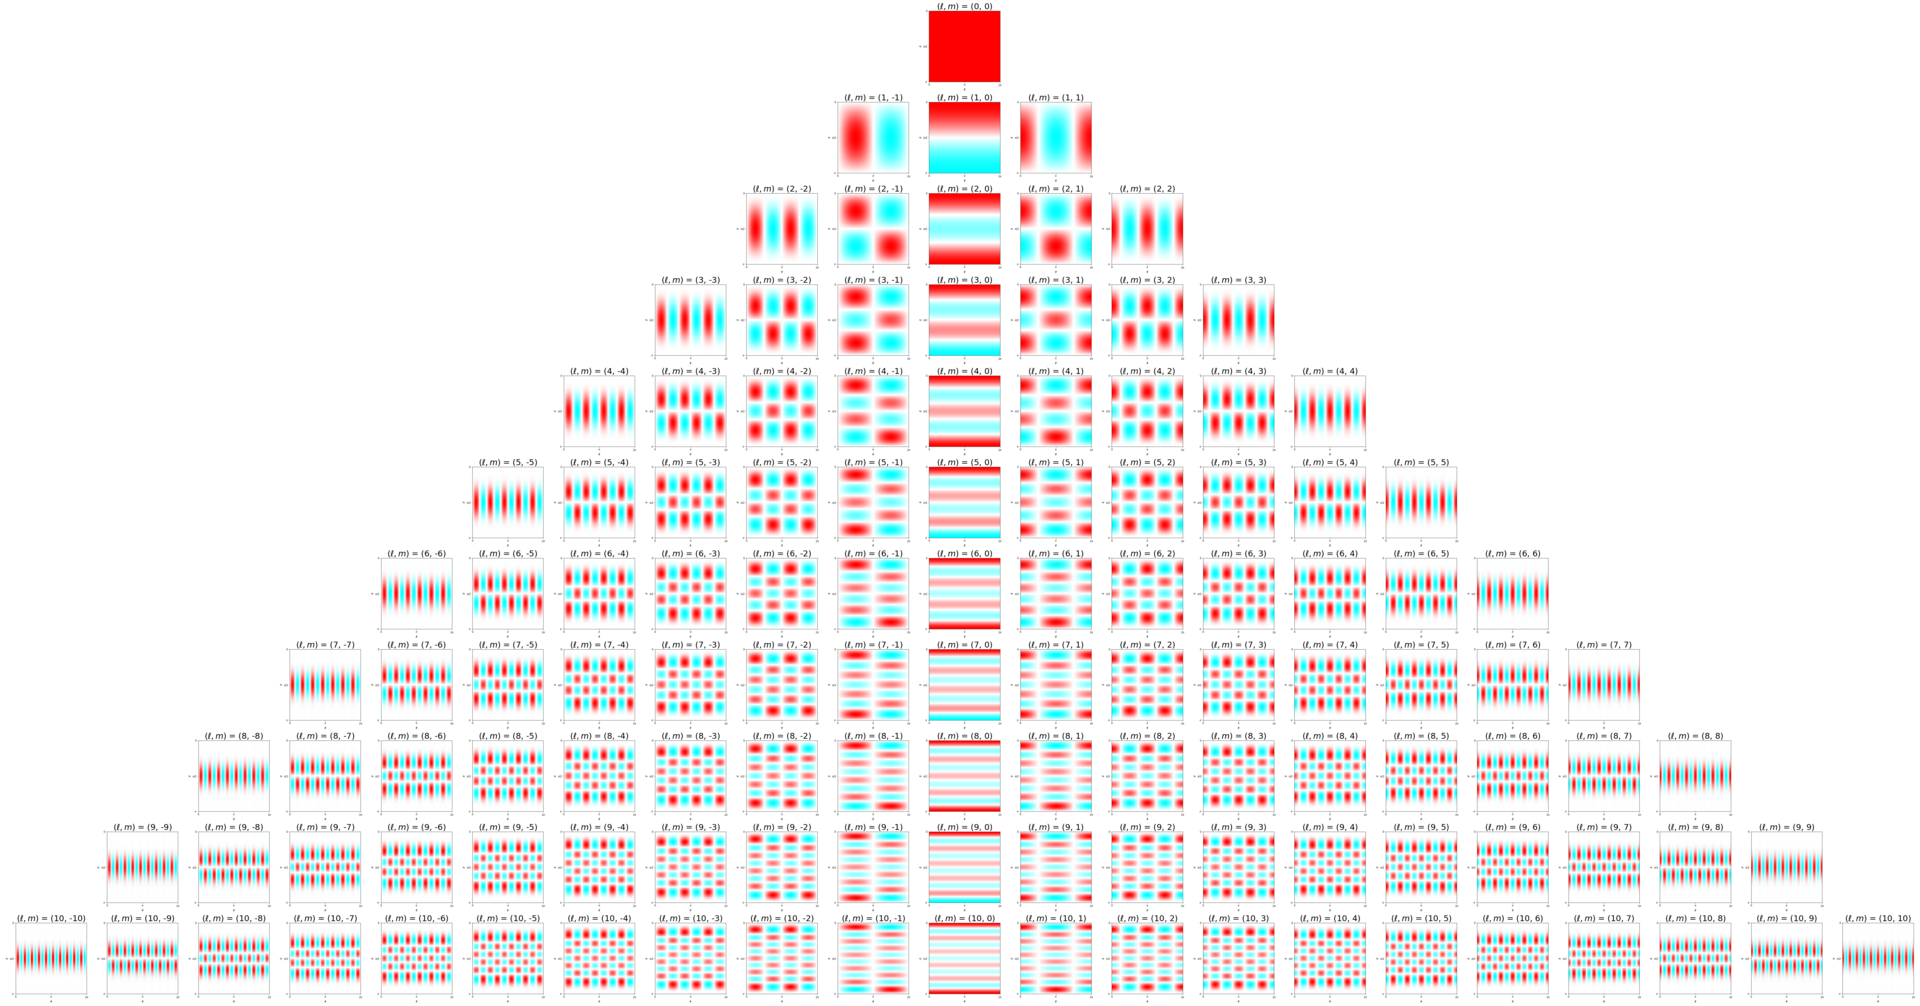
\includegraphics[width=1.0\textwidth]{images/Real_Spherical_Harmonics_Figure_Table_Complex_2D.png}
    \caption{The real spherical harmonics $Y_{lm}(\theta, \phi)$ in the 2D map.}
    \label{fig:real_spherical_harmonics}
\end{figure}

%\clearpage
\begin{figure}[!htbp]
    \centering
    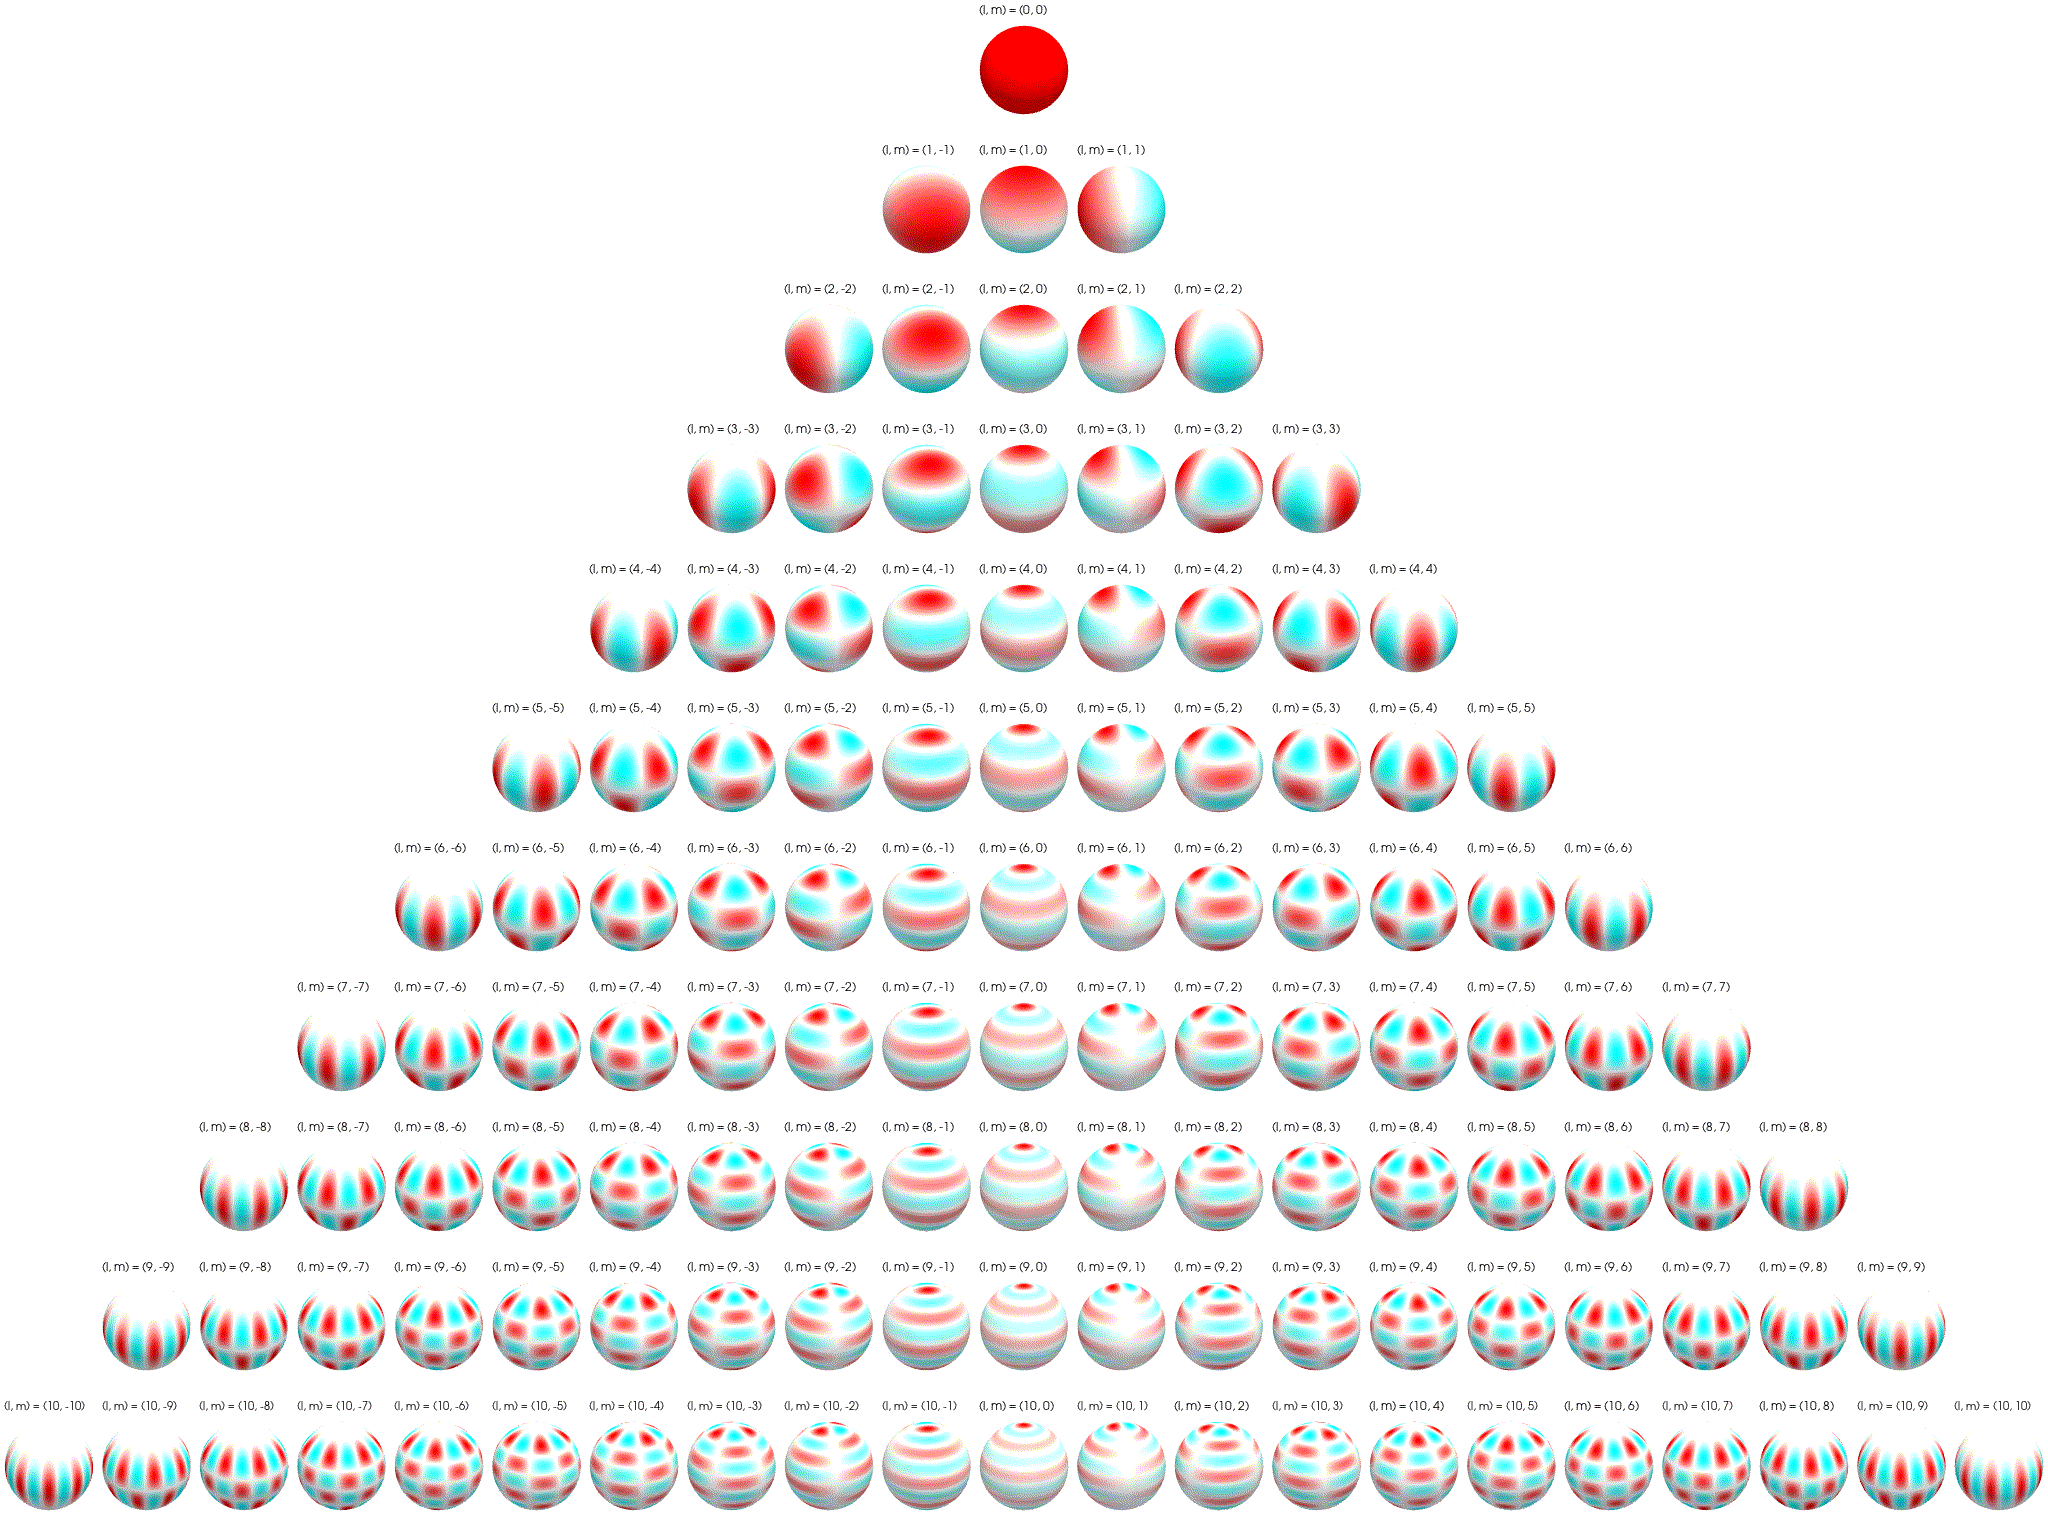
\includegraphics[width=0.9\textwidth]{images/Real_Spherical_Harmonics_Figure_Table_Complex_Polar_Plot.png}
    \caption{The real spherical harmonics $Y_{lm}(\theta, \phi)$ in the polar plot.}
    \label{fig:real_spherical_harmonics_polar}
\end{figure}

\begin{figure}[!htbp]
    \centering
    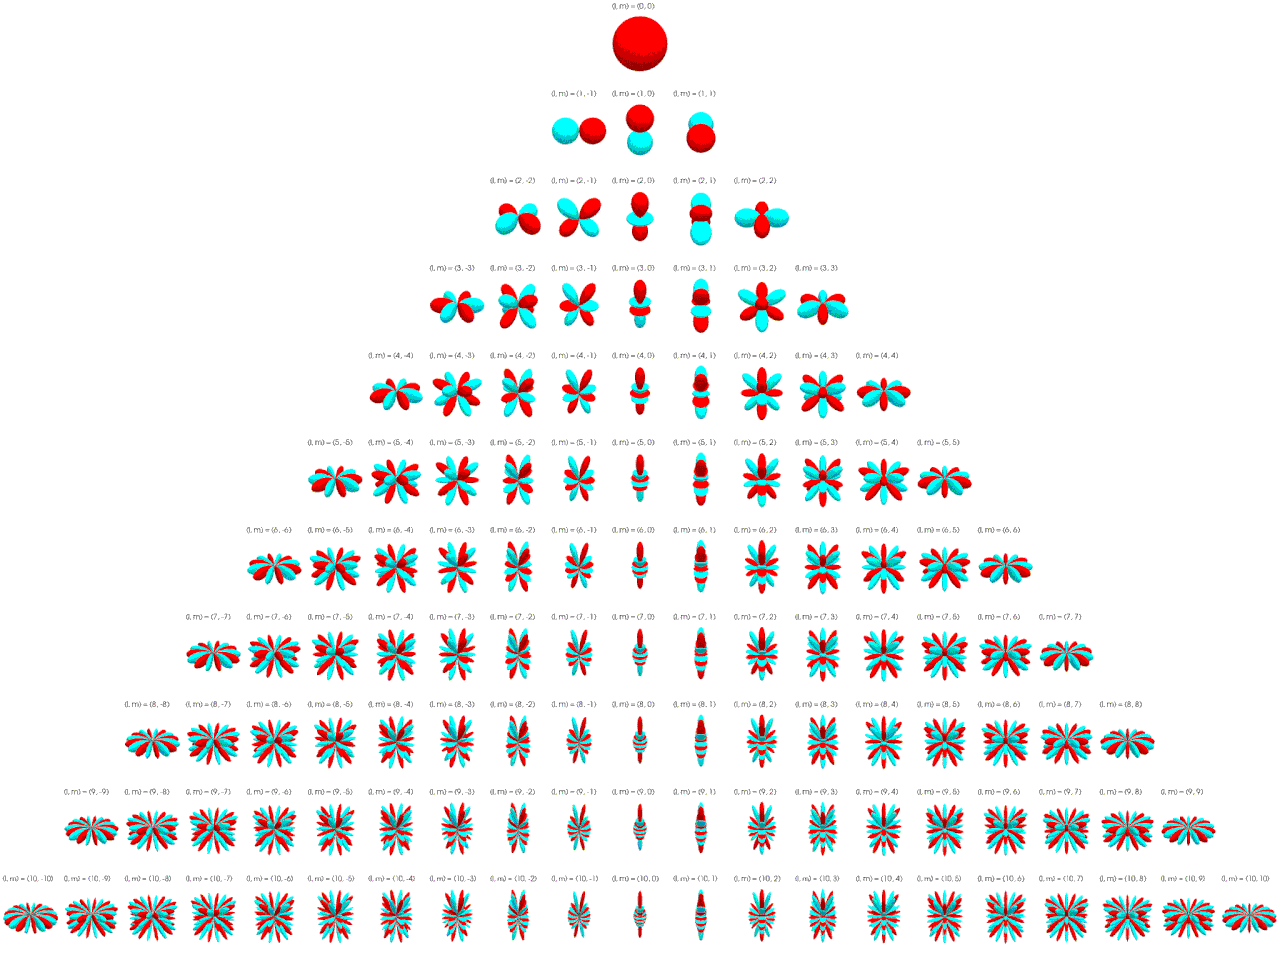
\includegraphics[width=0.9\textwidth]{images/Real_Spherical_Harmonics_Figure_Table_Complex_Radial_Magnitude.png}
    \caption{The real spherical harmonics $Y_{lm}(\theta, \phi)$ in the radial plot.}
    \label{fig:real_spherical_harmonics_radial}
\end{figure}






% -──────────────────────────────────────────────────────────────────────────────
\clearpage
%\bigskip \noindent \bigskip \noindent \bigskip \noindent
\subsection{Theoretical Power Spectrum}
\begin{intuition}
    In the previous section, we have shown that the temperature fluctuations can be described by the spherical harmonics, now it is time to analyze the statistical properties of the temperature fluctuations, which is the power spectrum. \\

    The \textbf{angular power spectrum} represents the variance of the temperature fluctuations exists in a specific angular scale, or in other words, it tells us "how rough" the CMB map when we look at patches of the sky with a specific angular size $\theta \approx 180^\circ / l$. Note that by cosmological principle, the CMB should be statistically isotropic, so we expect all orientations $m$ at the same scale $l$ should have the same average power spectrum $C_l$, and can be written as:
    \[
        C_l \equiv \frac{1}{2l + 1} \sum_{m=-l}^{l} \langle |a_{lm}|^2 \rangle
    \]
    which we sum over all $m$ for a fixed $l$ to get the average power spectrum at scale $l$. \\

    Further, we can let $\langle |a_{l,-l}|^2 \rangle = \dots = \langle |a_{l0}|^2 \rangle = \dots = \langle |a_{l,l}|^2 \rangle$ due to the isotropy of the CMB, and hence we can get:
    \[
        C_l = \langle |a_{lm}|^2 \rangle
    \]
\end{intuition}

\bigskip \noindent
\begin{remark}
    The power spectrum $C_l$ we defined here is a \textbf{theoretical power spectrum}, which is the average power spectrum we expect to see in the CMB map, thus in the equation, we used the bracket $\langle \cdot \rangle$ to represent the average over all possible realizations of the CMB map. 
\end{remark}

\bigskip \noindent
\begin{foundation}
    By the cosmological principle, for a different combination of $l$ and $m$, their coefficients $a_{lm}$ are independent and identically distributed random variables, which we have below properties:
    \begin{itemize}
        \item $\langle a_{lm} \rangle = 0$, which means the average of the coefficients is zero, which is expected as the temperature fluctuations should be around the average temperature $T_0$;
        \item if $l \neq l'$ or $m \neq m'$, then $\langle a_{lm} a_{l'm'}^* \rangle = \langle a_{lm} \rangle \langle a_{l'm'}^* \rangle = 0$, which means the coefficients are uncorrelated with each other;
        \item if $l = l'$ and $m = m'$, then $\langle a_{lm} a_{l'm'}^* \rangle = \langle |a_{lm}|^2 \rangle = C_l$, which means the variance of the coefficients is equal to the power spectrum at scale $l$.
    \end{itemize} \\

    Therefore, we can get the average temperature variance at scale $l$ as:
    \begin{align*}
        \langle \left( \frac{\Delta T}{T_0} \right)^2 \rangle &= \langle \left( \sum_{l=0}^{\infty} \sum_{m=-l}^{l} a_{lm} Y_{lm}(\theta, \phi) \right) \left( \sum_{l'=0}^{\infty} \sum_{m'=-l'}^{l'} a_{l'm'}^* Y_{l'm'}^*(\theta, \phi) \right) \rangle \\
        &= \sum_{l=0}^{\infty} \sum_{m=-l}^{l} \sum_{l'=0}^{\infty} \sum_{m'=-l'}^{l'} \langle a_{lm} a_{l'm'}^* \rangle Y_{lm}(\theta, \phi) Y_{l'm'}^*(\theta, \phi) \\
        &= \sum_{l=0}^{\infty} \sum_{m=-l}^{l} C_l Y_{lm}(\theta, \phi) Y_{lm}^*(\theta, \phi) \\
        &= \sum_{l=0}^{\infty} C_l \sum_{m=-l}^{l} |Y_{lm}(\theta, \phi)|^2 \\
        &= \sum_{l=0}^{\infty} C_l \cdot \frac{2l + 1}{4\pi} \\
         &= \frac{1}{4\pi} \sum_{l=0}^{\infty} (2l + 1) C_l
    \end{align*}
\end{foundation}

%% average temperature variance
\bigskip \noindent
\begin{theory}
    The average temperature variance at scale $l$ can be expressed as:
    \[
        \langle \left( \frac{\Delta T}{T_0} \right)^2 \rangle = \frac{1}{4\pi} \sum_{l=0}^{\infty} (2l + 1) C_l
    \]
    with $C_l = \langle |a_{lm}|^2 \rangle$ is the theoretical power spectrum at scale $l$.
\end{theory}

% -──────────────────────────────────────────────────────────────────────────────
\bigskip \noindent \bigskip \noindent \bigskip \noindent
\subsection{Observed Power Spectrum}
\begin{intuition}
    However, in reality, we can only observe one realization of the CMB map, which means we can only get one set of coefficients $a_{lm}$, and hence we can only get one set of power spectrum. Therefore, we need to define the \textbf{observed power spectrum} as:
    \[
        \hat{C}_l = \frac{1}{2l + 1} \sum_{m=-l}^{l} |a_{lm}|^2
    \]
    which is the power spectrum we can get from the observed CMB map. \\
\end{intuition}

\bigskip \noindent
\begin{foundation}
    Again, we can calculate the variance of the temperature fluctuations at scale $l$ using the observed power spectrum:
    \small
    \begin{align*}
        \frac{1}{4\pi} \int \left( \frac{\Delta T}{T_0} \right)^2 d\Omega &= \frac{1}{4\pi} \int \left( \sum_{l=0}^{L} \sum_{m=-l}^{l} a_{lm} Y_{lm}(\theta, \phi) \right) \left( \sum_{l'=0}^{L} \sum_{m'=-l'}^{l'} a_{l'm'}^* Y_{l'm'}^*(\theta, \phi) \right) d\Omega \\
        &= \frac{1}{4\pi} \sum_{l=0}^{L} \sum_{m=-l}^{l} \sum_{l'=0}^{L} \sum_{m'=-l'}^{l'} a_{lm} a_{l'm'}^* \int Y_{lm}(\theta, \phi) Y_{l'm'}^*(\theta, \phi) d\Omega \\
        &= \frac{1}{4\pi} \sum_{l=0}^{L} \sum_{m=-l}^{l} |a_{lm}|^2 \\
        &= \frac{1}{4\pi} \sum_{l=0}^{L} (2l + 1) \hat{C}_l
    \end{align*}
    \normalsize

    Note here actually $a_{lm} a_{l'm'}^* \neq 0$ when $l \neq l'$ or $m \neq m'$ in a single realization, the reason why here we can just ignore those terms and simplified the summation into $\sum_{l=0}^{L} \sum_{m=-l}^{l} |a_{lm}|^2$ is because the orthogonality of the spherical harmonic basis. It isolates the diagonal terms and hence we can just focus on the diagonal terms when we calculate the variance of the temperature fluctuations.
\end{foundation}

\bigskip \noindent
\begin{theory}
    The variance of the temperature fluctuations at scale $l$ can be expressed as:
    \[
        \frac{1}{4\pi} \int \left( \frac{\Delta T}{T_0} \right)^2 d\Omega = \frac{1}{4\pi} \sum_{l=0}^{L} (2l + 1) \hat{C}_l
    \]  
    with $\hat{C}_l = \frac{1}{2l + 1} \sum_{m=-l}^{l} |a_{lm}|^2$ is the observed power spectrum at scale $l$. And L is the maximum scale we can observe, which is determined by the resolution of the CMB map.
\end{theory}

\bigskip \noindent
\begin{importantnote}
    The \textbf{observed power spectrum} $\hat{C}_l$ is an estimator of the \textbf{theoretical power spectrum} $C_l$, which means $\hat{C}_l$ is a random variable that depends on the specific realization of the CMB map we observed, be aware that $\hat{C}_l$ is not equal to $C_l$, and there is a statistical uncertainty in the estimation of $C_l$ by $\hat{C}_l$, which is called \textbf{cosmic variance}.
\end{importantnote}

% -──────────────────────────────────────────────────────────────────────────────
\clearpage
%\bigskip \noindent \bigskip \noindent \bigskip \noindent
\subsection{Cosmic variance}
\begin{intuition}
    Now lets define the variance of the difference between the observed power spectrum $\hat{C}_l$ and the theoretical power spectrum $C_l$ as:
    \[
        \sigma_{C_l}^2 = \langle (\hat{C}_l - C_l)^2 \rangle
    \]
    which is the variance of the estimation of $C_l$ by $\hat{C}_l$. This variance is called \textbf{cosmic variance}, which is the fundamental statistical uncertainty in the estimation of the power spectrum due to the fact that we can only observe one realization of the universe. \\

    By intuition, we can expect that the cosmic variance should be larger at larger scales (smaller $l$) because we have fewer independent modes to average over, and hence the estimation of $C_l$ is more uncertain. On the other hand, at smaller scales (larger $l$), we have more independent modes to average over, and hence the estimation of $C_l$ is more accurate, which means the cosmic variance should be smaller at smaller scales.
\end{intuition}

\bigskip \noindent
\begin{foundation}
    Start with the definition of the cosmic variance:
    \begin{align*}
        \sigma_{C_l}^2 &= \langle (\hat{C}_l - C_l)^2 \rangle \\
        &= \langle \hat{C}_l^2 - 2 \hat{C}_l C_l + C_l^2 \rangle \\
        &= \langle \hat{C}_l^2 \rangle - 2 C_l \langle \hat{C}_l \rangle + C_l^2 \\
        &= \langle \hat{C}_l^2 \rangle - C_l^2
    \end{align*} 

    Since:
    \[
        \langle \hat{C}_l \rangle = \langle \frac{1}{2l + 1} \sum_{m=-l}^{l} |a_{lm}|^2 \rangle = C_l
    \]
    we can write $\langle \hat{C}_l^2 \rangle$ as:
    \begin{align*}
        \langle \hat{C}_l^2 \rangle &= \frac{1}{(2l + 1)^2} \sum_{m=-l}^{l} \sum_{m'=-l}^{l} \langle |a_{lm}|^2 |a_{lm'}|^2 \rangle \\
    \end{align*} \\

    \pagebreak
    By assuming the CMB fluctuations are Gaussian random fields, we can get the following properties of the coefficients $a_{lm}$:
    \begin{itemize}
        \item $m = 0$ case, we have $\langle |a_{l0}|^2 \rangle = \sigma^2 = C_l$, and hence we can get: 
            \begin{align*}
                \langle |a_{l0}|^4 \rangle &= \frac{1}{\sqrt{2\pi} \sigma} \int_{-\infty}^{\infty} x^4 e^{-\frac{x^2}{2\sigma^2}} dx \\
                &= 3 \sigma^4 \\
                &= 3 C_l^2
            \end{align*}
        \item $m \neq 0$ case, let $a_{lm} = x + i y$, where $x$ and $y$ are independent Gaussian random variables with mean 0 and variance $\sigma^2 = C_l/2$, we can get:
            \begin{align*}
                \langle |a_{lm}|^4 \rangle &= \langle (x^2 + y^2)^2 \rangle \\
                &= \langle x^4 + 2 x^2 y^2 + y^4 \rangle \\
                &= 3 \sigma^4 + 2 \sigma^4 + 3 \sigma^4 \\
                &= 8 \sigma^4 \\
                &= 2 C_l^2
            \end{align*}
    \end{itemize}
    And we get:
    \begin{align*}
        \langle |a_{lm}|^2 \rangle &= C_l \\
        \langle |a_{lm}|^4 \rangle &= \begin{cases}
            3 C_l^2, & m = 0 \text{ (real case)} \\
            2 C_l^2, & m \neq 0 \text{ (complex case)}
        \end{cases}
    \end{align*}
    We can further simplify $\langle \hat{C}_l^2 \rangle$ in 2 cases:
    \begin{itemize}
        \item For $m = m'$,
        \begin{itemize}
            \item if $m = 0$, then $\langle |a_{l0}|^4 \rangle = 3 C_l^2$; The number of zero diagonal term $m$ is 1.
            \item if $m \neq 0$, then $\langle |a_{lm}|^4 \rangle = 2 C_l^2$; The number of non-zero diagonal terms $m$ is $2l$.
        \end{itemize}
        \item For $m \neq m'$, we have $\langle |a_{lm}|^2 |a_{lm'}|^2 \rangle = \langle |a_{lm}|^2 \rangle \langle |a_{lm'}|^2 \rangle = C_l^2$; The number of off-diagonal terms is $(2l + 1)^2 - 1 - 2l$.
    \end{itemize} \\

    Hence, we can get:
    \begin{align*}
        \sum_{m=-l}^{l} \sum_{m'=-l}^{l} \langle |a_{lm}|^2 |a_{lm'}|^2 \rangle &= (3 C_l^2) \cdot 1 + (2 C_l^2) \cdot 2l + C_l^2 \cdot ((2l + 1)^2 - 1 - 2l) \\
        &=  ( 3 + 4l + 4l^2 + 4l + 1 - 1 - 2l ) C_l^2 \\
        &= (4l^2 + 6l + 3) C_l^2 \\
        &= (2l + 3)(2l + 1) C_l^2
    \end{align*}
    As a result, we get $\langle \hat{C}_l^2 \rangle$ as:
    \begin{align*}
        \langle \hat{C}_l^2 \rangle &= \frac{1}{(2l + 1)^2} \sum_{m=-l}^{l} \sum_{m'=-l}^{l} \langle |a_{lm}|^2 |a_{lm'}|^2 \rangle \\
        &= \frac{1}{(2l + 1)^2} (2l + 3)(2l + 1) C_l^2 \\
        &= \frac{2l + 3}{2l + 1} C_l^2
    \end{align*}
    
    Therefore, the cosmic variance is:
    \begin{align*}
        \sigma_{C_l}^2 &= \langle (\hat{C}_l - C_l)^2 \rangle \\
        &= \langle \hat{C}_l^2 \rangle - C_l^2 \\
        &= \left( \frac{2l + 3}{2l + 1} - 1 \right) C_l^2 \\
        &= \frac{2}{2l + 1} C_l^2
    \end{align*}
\end{foundation}

\bigskip \noindent
\begin{theory}
    The cosmic variance can be expressed as:
    \[
        \sigma_{C_l}^2 = \langle (\hat{C}_l - C_l)^2 \rangle = \frac{2}{2l + 1} C_l^2
    \]
    And the equation matches our intuition that the cosmic variance is larger at larger scales (smaller $l$) and smaller at smaller scales (larger $l$).
\end{theory}

\bigskip \noindent
\begin{figure}[!htbp]
    \centering
    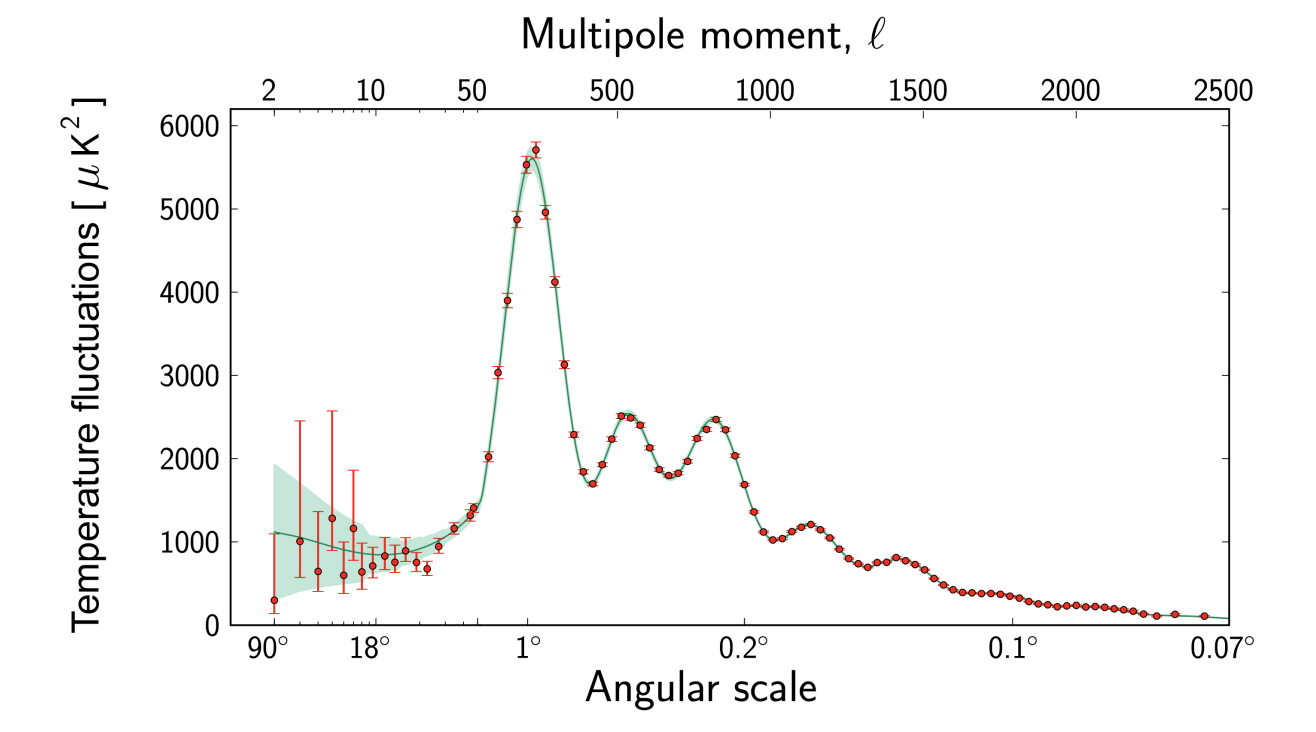
\includegraphics[width=0.8\textwidth]{images/angular_power_spectrum.png}
    \caption{The angular power spectrum of the CMB}
    \label{fig:angular_power_spectrum}
\end{figure}

\clearpage
\begin{extra}
    The above figure shows the angular power spectrum of the CMB. The x-axis represents the multipole moment $l$ (top) and the corresponding angular scale $\theta$ (bottom), related approximately by $\theta \approx 180^\circ / l$. The y-axis represents the scaled power spectrum, typically plotted as $\frac{l(l+1)C_l}{2\pi}$, which quantifies the variance of temperature fluctuations at scale $l$. \\

    The red dots with error bars represent the observed power spectrum $\hat{C}_l$ derived from CMB maps, while the green solid line represents the theoretical power spectrum predicted by the best-fit $\Lambda$CDM model. The green shaded region represents \textbf{cosmic variance}, the fundamental statistical uncertainty arising because we can only observe one realization of the universe. \\

    On the far left (low $l$), the curve is relatively flat. This is the \textbf{Sachs-Wolfe plateau}, which corresponds to super-horizon scales (larger than the causal horizon at recombination). These fluctuations are primordial, originating from quantum fluctuations stretched by inflation. \\

    In the middle region ($30 < l < 1000$), we see a series of \textbf{acoustic peaks}. These correspond to sound waves (oscillations) in the photon-baryon fluid before recombination.
    \begin{itemize}
        \item The \textbf{First Peak} ($l \approx 200$) represents the fundamental mode of oscillation—the maximum compression of the fluid. Its position at $1^\circ$ indicates that the universe is geometrically \textbf{flat}.
        \item The \textbf{Second Peak} represents the first rarefaction (expansion) phase.
        \item The \textbf{Third Peak} represents the second compression phase. The relative heights of these peaks (specifically the ratio of odd to even peaks) provide a precise measurement of the \textbf{baryon density} ($\Omega_b$) of the universe.
    \end{itemize} \\

    On the far right ($l > 1000$), the curve drops sharply. This is the \textbf{damping tail} (or Silk damping). On these very small scales, photons could diffuse through the plasma before recombination, effectively "smoothing out" the temperature fluctuations and erasing the signal. \\

    Further details about the meaning of above features will be discussed in next few sections, but here we just want to give a brief introduction about the shape of the angular power spectrum and its physical meaning.
\end{extra}



% =══════════════════════════════════════════════════════════════════════════════
\clearpage
\section{Acoustic Oscillations and Acoustic Peaks}
% -──────────────────────────────────────────────────────────────────────────────
%\bigskip \noindent \bigskip \noindent \bigskip \noindent
\subsection{Damped Harmonic Oscillator}
\begin{foundation}
    Recall about the equation of motion for a damped harmonic oscillator, in such a system, the total force is given 2 components: the restoring force $F_r = - k x$ and the damping force by friction $F_d = - b \frac{dx}{dt}$, where $k$ is the stiffness factor and $b$ is the viscous damping coefficient. The equation of motion can be written as:
    \[
        F = m \frac{d^2 x}{dt^2} = - k x - b \frac{dx}{dt}
    \]
    And can be rearranged into the standard form:
    \[
        \frac{d^2 x}{dt^2} + 2 \zeta \omega_0 \frac{dx}{dt} + \omega_0^2 x = 0
    \]
    where:
    \[
        \omega_0 = \sqrt{\frac{k}{m}}
    \] 
    is the natural angular frequency of the undamped system, and 
    \[
        \zeta = \frac{b}{2 \sqrt{km}}
    \]
    is the damping ratio.
\end{foundation}

\bigskip \noindent
\begin{theory} 
    By solving the damped harmonic oscillator equation, we can get the general solution as:
    \[
        x(t) = Ae^{-\zeta \omega_0 t} \sin(\sqrt{1 - \zeta^2} \omega_0 t + \phi)
    \]
    where $A$ is the amplitude of the oscillation, and $\phi$ is the phase constant. The term $e^{-\zeta \omega_0 t}$ represents the exponential decay of the amplitude due to damping, while the term $\sin(\sqrt{1 - \zeta^2} \omega_0 t + \phi)$ represents the oscillatory behavior of the system. \\
\end{theory}

\clearpage
%\bigskip \noindent
\begin{figure}[!htbp]
    \centering
    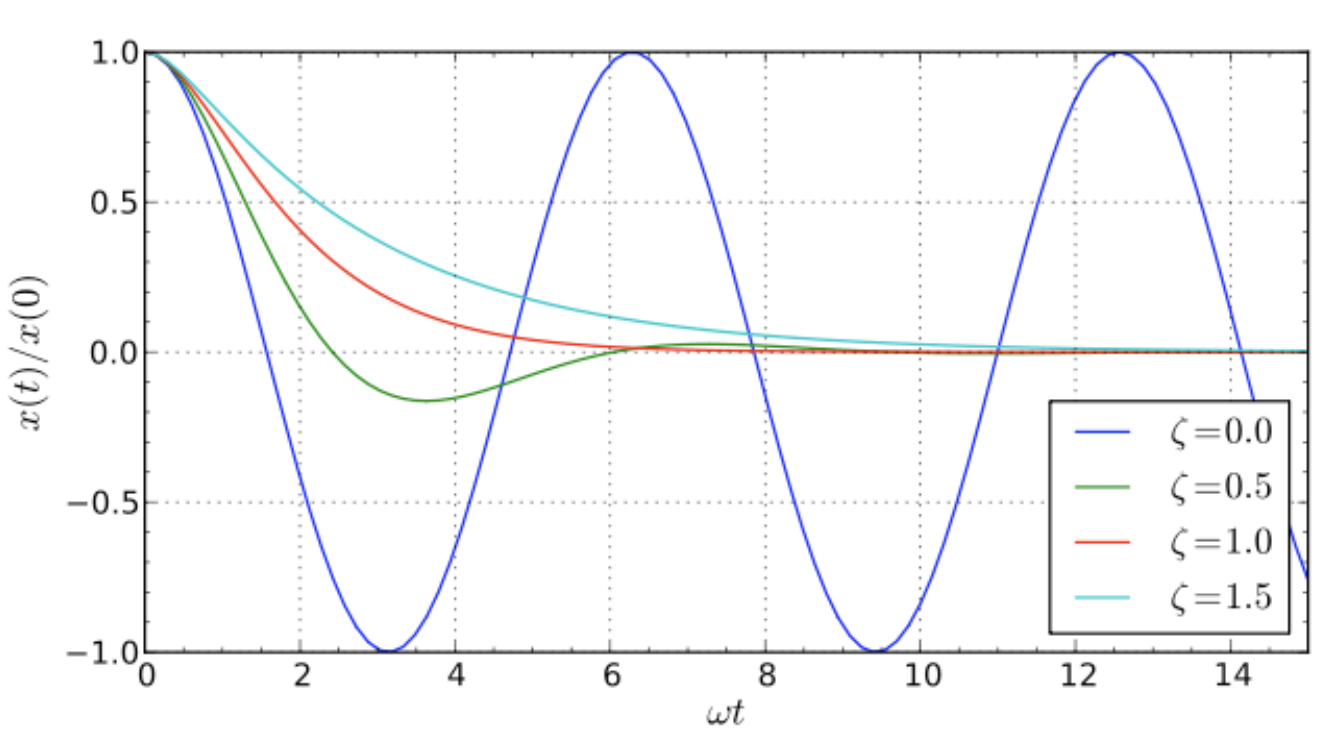
\includegraphics[width=0.8\textwidth]{images/damped_harmonic_oscillator.png}
    \caption{The motion of a damped harmonic oscillator for different values of the damping ratio $\zeta$.}
    \label{fig:damped_harmonic_oscillator}
\end{figure}

\begin{intuition}
    There is 4 types of damped harmonic oscillator:
    \begin{itemize}
        \item \textbf{Undamped} ($\zeta = 0$): the system oscillates indefinitely with a constant amplitude and a natural frequency $\omega_0$. A common example is a mass-spring system without any friction.
        \item \textbf{Underdamped} ($\zeta < 1, \zeta > 0$): the system oscillates with the amplitude gradually decreasing to zero over time. Besides, it oscillates(with a slightly lower frequency than the natural frequency $\omega_0$) because the damping is not strong enough to stop the oscillation immediately:
        \[
            \omega_u = \sqrt{1 - \zeta^2} \omega_0
        \]
        A common example is a mass-spring system with a small amount of friction.
        \item \textbf{Critically damped} ($\zeta = 1$): the system returns to equilibrium as quickly as possible without oscillating. It does not oscillate because the damping is just strong enough to prevent any oscillation. A common example is a door closer that brings the door to a stop without bouncing.
        \item \textbf{Overdamped} ($\zeta > 1$): the system returns to equilibrium in exponentially decaying without oscillating, but more slowly than in the critically damped case. The larger the damping ratio $\zeta$, the slower the system returns to equilibrium. A common example is a car shock absorber that is too stiff, causing the car to return to its normal position very slowly after hitting a bump.
    \end{itemize}
\end{intuition}

\bigskip \noindent
\begin{remark}
    We ignore the case of $\zeta < 0$ because it shows a system that gain energy from the environment, which will diverge and hence is not stable. 
\end{remark}







% -──────────────────────────────────────────────────────────────────────────────
\bigskip \noindent \bigskip \noindent \bigskip \noindent
\subsection{Acoustic Oscillations in CMB}
\begin{intuition}
    Before recombination, the universe is filled with a hot, dense plasma of photons, electrons, and baryons. The photons are tightly coupled to the electrons through Thomson scattering, and the electrons are coupled to the baryons through Coulomb interactions. This photon-baryon fluid can support sound waves (acoustic oscillations) due to the interplay between the pressure of the photons and the gravitational attraction of the baryons. \\

    The acoustic oscillations in the photon-baryon fluid before recombination can be described by a damped harmonic oscillator equation, where the restoring force is provided by the pressure of the photons, and the damping is caused by the expansion of the universe and the diffusion of photons (Silk damping). The solutions to this equation give rise to the characteristic peaks in the CMB power spectrum, known as acoustic peaks. \\

    Finally, after recombination, the photons decouple and the acoustic oscillations are frozen in, leaving an imprint on the CMB that we can observe today. 
\end{intuition}

\bigskip \noindent
\begin{foundation}
    considering a \textbf{fixed volume} bounded by surface, we can get the total number of photons in the volume as:
    \[
        N_\gamma(t) = \int_V n_\gamma(\vec{x},t) dV = \int_V n_\gamma(x,t) d^3 x
    \]
    At the same time, the net change of the number of photons in the volume is given by the flux of photons across the surface:
    \[
        \frac{dN_\gamma}{dt} = - \oint_S n_\gamma(\vec{x},t) \vec{v} \cdot d\vec{S}
    \]
    Then we can write the 2 equations together as:
    \begin{align*}
        \frac{d}{dt} \int_V n_\gamma(\vec{x},t) d^3 x &= - \oint_S n_\gamma(\vec{x},t) \vec{v} \cdot d\vec{S} \\
        \int_V \frac{\partial n_\gamma(\vec{x},t)}{\partial t} d^3 x &= - \oint_S n_\gamma(\vec{x},t) \vec{v} \cdot d\vec{S}
    \end{align*}

    By applying the divergence theorem:
    \[
        \oint_S n_\gamma(\vec{x},t) \vec{v} \cdot d\vec{S} = \int_V \nabla \cdot (n_\gamma(\vec{x},t) \vec{v}) d^3 x
    \]
    we have:
    \begin{align*}
        \int_V \frac{\partial n_\gamma(\vec{x},t)}{\partial t} d^3 x &= - \int_V \nabla \cdot (n_\gamma(\vec{x},t) \vec{v}) d^3 x \\
        \int_V \left( \frac{\partial n_\gamma(\vec{x},t)}{\partial t} + \nabla \cdot (n_\gamma(\vec{x},t) \vec{v}) \right) d^3 x &= 0
    \end{align*}
    Since the above equation holds for any arbitrary volume, we can get the continuity equation for the number density of photons as:
    \[
        \frac{\partial n_\gamma(\vec{x},t)}{\partial t} + \nabla \cdot (n_\gamma(\vec{x},t) \vec{v}) = 0
    \]
\end{foundation}

\bigskip \noindent
\begin{foundation}
    The above equation assume a fixed volume, but we know that the \textbf{universe is expanding}, so we need to consider the scale factor in the equation:
    \[
        N_\gamma(t) = n_\gamma(t) a^3(t) = \text{constant}
    \]
    Then by conservation of the number of photons, we can get:
    \begin{align*}
        \frac{dN_\gamma}{dt} &= 0\\
        \frac{d}{dt} (n_\gamma(t) a^3(t)) &= 0 \\
        \dot{n}_\gamma(t) a^3(t) + 3 n_\gamma(t) a^2(t) \dot{a}(t) &= 0\\
        \dot{n}_\gamma(t) + 3 n_\gamma(t) \frac{\dot{a}(t)}{a(t)} &= 0 \\
        \dot{n}_\gamma(t) + 3 n_\gamma(t) H(t) &= 0
    \end{align*}
    And substituting the above equation into the continuity equation, we can get:
    \begin{align*}
        \frac{dN_\gamma}{dt} &= -\oint_S n_\gamma(\vec{x},t) \vec{v} \cdot d\vec{S} \\
        \int_V \left( \frac{\partial \left( n_\gamma(\vec{x},t) a^3(t) \right)}{\partial t} + \nabla \cdot (n_\gamma(\vec{x},t) \vec{v}) \right) d^3 x &= 0 \\
        \int_V \left( \dot{n}_\gamma(t) + 3 n_\gamma(t) H(t) + \nabla \cdot (n_\gamma(\vec{x},t) \vec{v}) \right) d^3 x &= 0 \\
        \dot{n}_\gamma(t) + 3 n_\gamma(t) H(t) + \nabla \cdot (n_\gamma(\vec{x},t) \vec{v}) &= 0
    \end{align*}
\end{foundation}

\bigskip \noindent
\begin{theory}
    The continuity equation for the number density of photons in an expanding universe can be expressed as:
    \[
        \dot{n}_\gamma(t) + 3 n_\gamma(t) H(t) + \nabla \cdot (n_\gamma(\vec{x},t) \vec{v}) = 0
    \]
    where $n_\gamma(t)$ is the number density of photons, $H(t)$ is the Hubble parameter, and $\vec{v}$ is the velocity field of the photons. \\

    In a special case of static universe where $H(t) = 0$, the above equation reduces to the standard continuity equation:
    \[
        \dot{n}_\gamma(t) + \nabla \cdot (n_\gamma(\vec{x},t) \vec{v}) = 0
    \]
\end{theory}

\bigskip \noindent
\begin{foundation}
    As we only interested in the small scale perturbations of the number density of photons, we can linearize the number desnity of photons as:
    \[
        n_\gamma(\vec{x},t) \approx \bar{n}_\gamma(t) + \delta n_\gamma(\vec{x},t)
    \]
    where $\bar{n}_\gamma(t)$ is the average number density of photons, and $\delta n_\gamma(\vec{x},t)$ is the perturbation of the number density of photons. Substituting the above equation into the continuity equation, we can get:
    \small
    \begin{align*}
        \dot{\bar{n}}_\gamma(t) + \dot{\delta n}_\gamma(\vec{x},t) + 3 (\bar{n}_\gamma(t) + \delta n_\gamma(\vec{x},t)) H(t) + \nabla \cdot ((\bar{n}_\gamma(t) + \delta n_\gamma(\vec{x},t)) \vec{v}) &= 0 \\
        \dot{\bar{n}}_\gamma(t) + 3 \bar{n}_\gamma(t) H(t) + \dot{\delta n}_\gamma(\vec{x},t)   + 3 \delta n_\gamma(\vec{x},t) H(t) + \nabla \cdot (\bar{n}_\gamma(t) \vec{v}) + \nabla \cdot (\delta n_\gamma(\vec{x},t) \vec{v}) &= 0
    \end{align*}
    \normalsize
    Since $\bar{n}_\gamma(t)$ is the average number density of photons, it should satisfy the background continuity equation:
    \[
        \dot{\bar{n}}_\gamma(t) + 3 \bar{n}_\gamma(t) H(t) = 0
    \]
    we can simplify the above equation into:
    \[
        \dot{\delta n}_\gamma(\vec{x},t) + 3 \delta n_\gamma(\vec{x},t) H(t) + \nabla \cdot (\bar{n}_\gamma(t) \vec{v}) + \nabla \cdot (\delta n_\gamma(\vec{x},t) \vec{v}) = 0 
    \] \\

    Furthermore, consider the last 2 terms in the above equation:
    \begin{itemize}
        \item $\nabla \cdot (\bar{n}_\gamma(t) \vec{v})$: since $\bar{n}_\gamma(t)$ is only a function of time, we can take it out of the divergence operator, and we have $\nabla \cdot (\bar{n}_\gamma(t) \vec{v}) = \bar{n}_\gamma(t) \nabla \cdot \vec{v}$. We keep this term because $\nabla \cdot \vec{v}$ is a first order perturbation, and hence it is not negligible in the linear approximation.
        \item $\nabla \cdot (\delta n_\gamma(\vec{x},t) \vec{v})$: since both $\delta n_\gamma(\vec{x},t)$ and $\vec{v}$ are small perturbations, we can ignore the second order term $\nabla \cdot (\delta n_\gamma(\vec{x},t) \vec{v})$ in the linear approximation.
    \end{itemize} \\

    At the sametime, we compare the magnitude of the remaining 3 terms, we know that $\dot{\delta n}_\gamma(\vec{x},t)$ is the time derivative of the perturbation, which is expected to be of the same order of magnitude as $\delta n_\gamma(\vec{x},t)$; \\
    And $3 \delta n_\gamma(\vec{x},t) H(t)$ is the expansion term, which is expected to be smaller than $\dot{\delta n}_\gamma(\vec{x},t)$ because the expansion of the universe is relatively slow compared to the time evolution of the perturbations. Therefore, we can also ignore the expansion term $3 \delta n_\gamma(\vec{x},t) H(t)$ in the linear approximation. \\

    As a result, we can simplify the above equation into:
    \begin{align*}
        \dot{\delta n}_\gamma(\vec{x},t) + \bar{n}_\gamma(t) \nabla \cdot \vec{v} &\approx 0 \\
        \dot{\delta n}_\gamma(\vec{x},t) &\approx - \bar{n}_\gamma(t) \nabla \cdot \vec{v} \\
        \frac{\dot{\delta n}_\gamma(\vec{x},t)}{\bar{n}_\gamma(t)} &\approx - \nabla \cdot \vec{v}
    \end{align*} \\

    Recall that $n_\gamma = \frac{2 \zeta(3)}{\pi^2} T^3$, we can get $\bar{n}_\gamma(t) = C T^3(t)$, and hence we can write the above equation as:
    \[
        \frac{\delta n_\gamma(\vec{x},t)}{\bar{n}_\gamma(t)} = \frac{3C T_0^2(t) \delta T(\vec{x},t)}{C T_0^3(t)} = 3 \frac{\delta T(\vec{x},t)}{T_0(t)} \equiv 3 \Theta(\vec{x},t)
    \]
    Substituting the above equation into the previous equation, we can get:
    \[
        \dot{\Theta}(\vec{x},t) \approx - \frac{1}{3} \nabla \cdot \vec{v}
    \]  
\end{foundation}

\bigskip \noindent
\begin{theory}
    By considering the small scale perturbations of the number density of photons in an expanding universe, we can derive the following equation:
    \[
        \dot{\Theta}(\vec{x},t) = - \frac{1}{3} \nabla \cdot \vec{v}
    \]
    where:\[
        \Theta(\vec{x},t) = \frac{\delta T(\vec{x},t)}{T_0(t)} = \frac{1}{3} \frac{\delta n_\gamma(\vec{x},t)}{\bar{n}_\gamma(t)}
    \]
    is the temperature perturbation, and $\vec{v}$ is the velocity field of the photons. 
\end{theory}

\clearpage
%\bigskip \noindent
\begin{foundation}
    Fourier transforming the temperature perturbation equation:
    \begin{align*}
        \dot{\Theta}(\vec{k},t) &\approx - \frac{1}{3} \nabla \cdot \vec{v}(\vec{k},t) \\
        \dot{\Theta}(\vec{k},t) &\approx - \frac{1}{3} i \vec{k} \cdot \vec{v}(\vec{k},t) \\
        \dot{\Theta}(\vec{k},t) &\approx - \frac{1}{3} i k v(\vec{k},t)
    \end{align*} \\

    At same time, we can also derive the Euler equation for the velocity field of the photons. Ignoring gravity and expansion of universe first, so that we can focus on the small scale oscillatory behavior of the system:
    \begin{align*}
        \dot{v} &= - \frac{\nabla \delta P_\gamma}{\rho_\gamma + P_\gamma} \\
        \dot{v} &= - \frac{\nabla \delta P_\gamma}{\frac{4}{3} \rho_\gamma} \\
    \end{align*}
    While the pressure perturbation $\delta P_\gamma$ is in terms of $\Theta$ as:
    \begin{align*}
        \frac{\delta P_\gamma}{\bar{P}_\gamma} &= 4 \frac{\delta T}{T_0} = 4 \Theta \\
        \delta P_\gamma &= 4 \Theta \bar{P}_\gamma = 4 \Theta \frac{1}{3} \bar{\rho}_\gamma = \frac{4}{3} \Theta \bar{\rho}_\gamma\\
    \end{align*}
    Substituting the above equation into the Euler equation, we can get:
    \begin{align*}
        \dot{v} &= - \frac{\nabla \delta P_\gamma}{\frac{4}{3} \rho_\gamma} \\
        \dot{v} &= - \frac{\nabla \left( \frac{4}{3} \Theta \bar{\rho}_\gamma \right)}{\frac{4}{3} \rho_\gamma} \\
        \dot{v} &= - \nabala \Theta \\
        \dot{v} &= - i k \Theta
    \end{align*} \\

    Finally, by taking the time derivative of the temperature perturbation equation, we can get:
    \begin{align*}
        \ddot{\Theta}(\vec{k},t) &\approx - \frac{1}{3} i k \dot{v}(\vec{k},t) \\
        \ddot{\Theta}(\vec{k},t) + \frac{1}{3} k^2 \Theta(\vec{k},t) &\approx 0
    \end{align*}
\end{foundation}

\bigskip \noindent
\begin{theory}
    We can derive the equation of temperature perturbation into a simple harmonic oscillator equation as:
    \[
        \ddot{\Theta}(\vec{k},t) + c_s^2 k^2 \Theta(\vec{k},t) = 0
    \]
    with the sound speed $c_s = \frac{1}{\sqrt{3}}$, and hence $\omega_0 = c_s k = \frac{k}{\sqrt{3}}$. \\

    By comparing the equation and the harmonic oscillator equation, we can see that it miss the damping term(friction term) in the equation, we will discuss more about this in next few sections.
\end{theory}

\bigskip \noindent
\begin{remark}
    Although it is oscillation of photon-baryon fluid, we can still call it "acoustic oscillation" because the sound waves in the photon-baryon fluid are analogous to the sound waves in air, and they both involve the propagation of pressure perturbations through a medium. The term "acoustic" is used to emphasize the wave-like nature of these oscillations and their role in shaping the CMB power spectrum.
\end{remark}

\bigskip \noindent
\begin{importantnote}
    The above model is an oversimplified model that ignores the damping effect and effect of baryons, but it can still capture the essential physics and provide a good intuition about the acoustic oscillations in the photon-baryon fluid before recombination. Therefore, we will still use the above model to discuss about the acoustic peaks in the power spectrum, and we will discuss more about the damping effect and effect of baryons in next few sections.
\end{importantnote}



% -──────────────────────────────────────────────────────────────────────────────
%\clearpage
\bigskip \noindent \bigskip \noindent \bigskip \noindent
\subsection{Acoustic Peaks in the Power Spectrum}
\begin{intuition}
    After making the model of acoustic oscillation in the photon-baryon fluid, we can now try to understand how the acoustic peaks in the CMB power spectrum are formed. The acoustic peaks correspond to the modes of oscillation that have reached either maximum compression or maximum rarefaction at the time of recombination. These modes will leave a strong imprint on the CMB power spectrum, resulting in the characteristic peaks that we observe. \\
\end{intuition}

%\bigskip \noindent
\clearpage
\begin{foundation}
    Recall the relationship between physical wavelength $\lambda$ and the comoving wavelength $\lambda_c$:
    \[
        \lambda = a(t) \lambda_c
    \]
    as $k \propto \frac{1}{\lambda}$, we can get the relationship between physical angular wave number $k$ and comoving angular wave number $k^c$ as:
    \begin{align*}
        k^c &= a(t) k
    \end{align*}

    Let $\omega_0$ be the angular frequency, and $c_s$ be the sound speed, we get:
    \begin{align*}
        \omega_0 &= c_s k \\
        \omega_0 &= c_s \frac{k^c}{a} \\
        \omega_0 &= \frac{c_s }{a} k^c \\
        \omega_0 &= c_s^c k^c
    \end{align*}
    where $c_s^c = \frac{c_s}{a}$ is the comoving sound speed. \\

    Then, recall the relationship between agnular scale $\theta$ and multipole moment $l$:
    \[
        \theta = \frac{2\pi}{l}
    \]
    And with long enough distance assumption, we let $\frac{\lambda}{d_A} = \tan \theta \approx \theta$, which $d_A$ is the angular diameter distance, so we can get:
    \begin{align*}
        \frac{\lambda}{d_A} &= \frac{2\pi}{l} \\
        \frac{2\pi}{k d_A} &= \frac{2\pi}{l} \\
        k &= \frac{l}{d_A} \\
        k^c &= l \frac{a}{d_A} \\
        k^c &= \frac{l}{d_A^c}
    \end{align*}
    where $d_A^c = \frac{d_A}{a}$ is the comoving angular diameter distance. \\

    Substituting the above equation back to the $\omega_0$ equation, and considering the $i$-th mode of the oscillation, we can get:
    \begin{align*}
        \omega_0^i &= c_s^c k^c_i \\
        \omega_0^i &= c_s^c \frac{l_i}{d_A^c} \\
        \omega_0^i &= \frac{c_s^c}{d_A^c} l(k_i)
    \end{align*}
    where $l(k_i) = l_i$ is the mode number of the oscillation.
\end{foundation}

\begin{theory}
    The $i$-th mode of angular wave number $k_i$ in the acoustic oscillation corresponds to a multipole moment $l_i$ in the CMB power spectrum, and the relationship can be expressed as:
    \[
        k^c_i = \frac{l_i}{d_A^c}
    \]
    where $d_A^c$ is the comoving angular diameter distance. \\

    And hence, the angular frequency of the $i-th$ mode can be expressed as:
    \[
        \omega_0^i = \frac{c_s^c}{d_A^c} l(k_i)
    \]
    where $c_s^c$ is the comoving sound speed, and $l(k_i)$ is the mode number of the oscillation.
\end{theory}

\begin{figure}[!htbp]
    \centering
    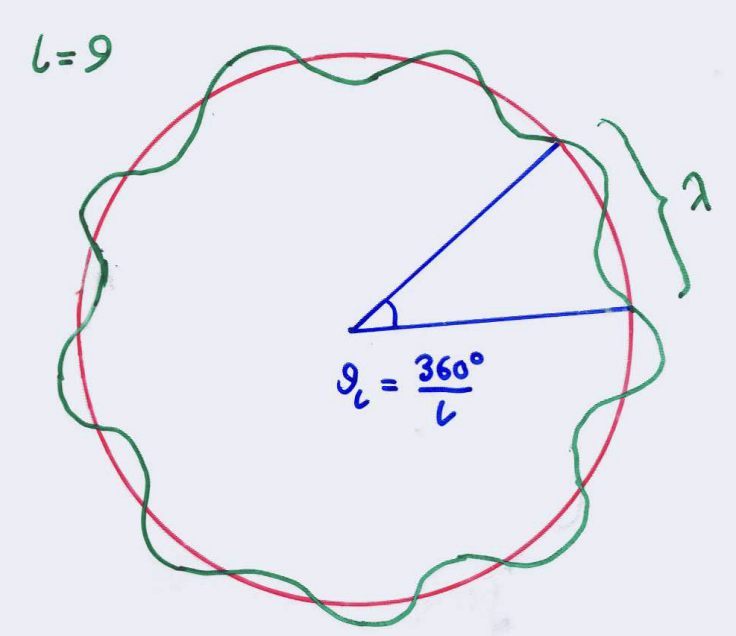
\includegraphics[width=0.5\textwidth]{images/angle_multipoles.png}
    \caption{The rough relationship between the angular scale $\theta$ and the multipole moment $l$.}
    \label{fig:angle_multipoles}
\end{figure}

\bigskip \noindent
\begin{foundation}
    Now lets define the sound horizon $r_s^c$ as the comoving distance that a sound wave can travel from the beginning of the universe to the time of recombination $t_{rec}$:
    \begin{align*}
        r_s^c(t_{rec}) &= \int_0^{t_{rec}} c_s^c dt = \int_0^{t_{rec}} \frac{c_s}{a} dt \\
    \end{align*}
    
    Further, assume that for a specific mode $i$, it achieves the maximum compression or maximum rarefaction at the time of recombination $t_{rec}$, its angular frequency $\omega_0^i$ must be an integer multiple of $\pi$:
    \begin{align*}
        \omega_0^i t_{rec} &= n \pi \quad, n = 1, 2, 3, \dots \\
    \end{align*}
    And hence:
    \begin{align*}
        \frac{c_s^c}{d_A^c} l(k_i) t_{rec} &= n \pi \\
        l(k_i) &= n \pi \frac{d_A^c}{c_s^c t_{rec}} \\
        l(k_i) &\approx n \pi \frac{d_A^c}{r_s^c(t_{rec})} \\
        l(k_i) &= n l_A
    \end{align*}
    where we used the approximation that $r_s^c(t_{rec}) \approx c_s^c t_{rec}$, and we defined the acoustic scale $l_A$ as:
    \[
        l_A = \pi \frac{d_A^c}{r_s^c(t_{rec})} = \frac{\pi}{\theta_s} \sim 220
    \]
    with $\theta_s$ is sound horizon angle, which is the angular size of the sound horizon at the time of recombination, and it is defined as:
    \[
        \theta_s = \frac{r_s^c(t_{rec})}{d_A^c}
    \]
\end{foundation}

\begin{theory}
    The multipole moments of the acoustic peaks in the CMB power spectrum can be expressed as integer multiples of the acoustic scale $l_A$:
    \[
        l(k_i) = n l_A
    \]
    where $n$ is a positive integer, and $l_A$ is defined as:
    \[
        l_A = \pi \frac{d_A^c}{r_s^c(t_{rec})} = \frac{\pi}{\theta_s} \sim 220
    \]
    with $d_A^c$ is the comoving angular diameter distance, and $r_s^c(t_{rec})$ is the comoving sound horizon at the time of recombination.
\end{theory}

\clearpage
%\bigskip \noindent
\begin{intuition}
    The above equation shows that the positions of the acoustic peaks in the CMB power spectrum are determined by 2 important factors: the comoving angular diameter distance $d_A^c$ and the comoving sound horizon $r_s^c(t_{rec})$. \\
    
    The comoving angular diameter distance $d_A^c$ depends on the geometry of the universe and the expansion history, while the comoving sound horizon $r_s^c(t_{rec})$ depends on the physical conditions of the early universe, such as the baryon density and the radiation density. \\
    
    Therefore, by measuring the positions of the acoustic peaks in the CMB power spectrum, we can infer important information about the geometry and composition of the universe.
\end{intuition}

\begin{figure}[!htbp]
    \centering
    \begin{tikzpicture}[scale=1.0, >=Latex]
        % Vertices of the right triangle
        \coordinate (O) at (0,0);      % Observer
        \coordinate (B) at (8,0);      % Base endpoint on LSS
        \coordinate (T) at (8,2.8);    % Top endpoint (sound horizon)

        % Triangle edges
        \draw[thick] (O) -- (B) -- (T) -- cycle;

        % Right-angle marker at B
        \draw[thick] (7.65,0) -- (7.65,0.35) -- (8,0.35);

        % Observer eye icon (simple stylized)
        \fill (O) circle (1.2pt);
        %\draw[thick] (-0.65,0.16) .. controls (-0.35,0.45) and (0.35,0.45) .. (0.65,0.16);
        %\draw[thick] (-0.65,-0.16) .. controls (-0.35,-0.45) and (0.35,-0.45) .. (0.65,-0.16);
        \fill (0,0) circle (1.8pt);

        % Labels for points
        \node[below left] at (O) {Observer};
        \node[below] at (B) {Last-scattering surface};

        % Side labels
        \node[below] at (4,0) {$d_A^c$};
        \node[right] at (8,1.4) {$r_s^c(t_{rec})$};

        % Angle arc at observer
        \draw[thick] (1.2,0) arc[start angle=0,end angle=19.3,radius=1.2];
        \node at (1.85,0.25) {$\theta_s$};

        % Optional line-of-sight note
        \node[below] at (4,-0.75) {line of sight};
    \end{tikzpicture}
    \caption{Analogy of right-triangle geometry for the sound-horizon angle.}
    \label{fig:sound_horizon_triangle}
\end{figure}


% -──────────────────────────────────────────────────────────────────────────────
\bigskip \noindent \bigskip \noindent \bigskip \noindent
\subsection{Comoving Diameter Distance}
\begin{intuition}
    The comoving angular diameter distance $d_A^c(t_{rec})$ shows the comoving distance that light travels from the last-scattering surface to us. Note it is dependent on spacetime evolution \textbf{after} recombination.
\end{intuition}

\bigskip \noindent
\begin{foundation}
    In general case where space can be flat or non-flat, we defined:
    \[
        \Omega_0 = \Omega_{m,0} + \Omega_{\Lambda,0} + \Omega_{r,0} + \Omega_{k,0}
    \]
    As radiation-dominated era end much earlier than recombination (around 50,000 years after the big bang), we can ignore the contribution of radiation to the total energy density of the universe at the time of recombination, and hence we can write $\Omega_0$ as:
    \[
        \Omega_0 = \Omega_{m,0} + \Omega_{\Lambda,0} + \Omega_{k,0}
    \]
    with $\Omega_{k,0} = 1 - \Omega_{m,0} - \Omega_{\Lambda,0}$ is the curvature density parameter. \\

    Using above definition, we can write the comoving angular diameter distance as:
    \begin{align*}
        d_A^c(t_{rec}) &= \int_{t_{rec}}^{t_0} \frac{dt}{a(t)} \\
        d_A^c(a_{rec}) &= \int_{a_{rec}}^{a_0} \frac{da}{a^2 H(a)} \\
         &= \int_{a_{rec}}^{a_0} \frac{da}{a^2 H_0 \sqrt{\Omega_{m,0} a^{-3} + \Omega_{\Lambda,0} + \Omega_{k,0} a^{-2}}} \\
         &= \frac{1}{H_0} \int_{a_{rec}}^{a_0} \frac{da}{a^2 \sqrt{\Omega_{m,0} a^{-3} + \Omega_{\Lambda,0} + (\1 - \Omega_{m,0} - \Omega_{\Lambda,0}) a^{-2}}} \\
         &= \frac{1}{H_0} \int_{a_{rec}}^{a_0} \frac{da}{a^2 \sqrt{\Omega_{m,0} (a^{-3} - a^{-2}) + \Omega_{\Lambda,0} (1 - a^{-2}) + a^{-2}}} \\
         &= \frac{1}{H_0} \int_{a_{rec}}^{a_0} \frac{da}{\sqrt{\Omega_{m,0} (a - a^2) - \Omega_{\Lambda,0} (a^2 - a^4) + a^2}} \\
         &= \frac{1}{H_0} \int_{a_{rec}}^{a_0} \frac{da}{\sqrt{\Omega_{0}^{'}(a - a^2) - \Omega_{\Lambda,0} (a - a^4) + a^2}}
    \end{align*}
    if we define $\Omega_{0}^{'} = 1 - \Omega_{m,0} - \Omega_{\Lambda,0}$ as the curvature density parameter.
\end{foundation}

\bigskip \noindent
\begin{theory}
    The comoving angular diameter distance from the last-scattering surface to us can be expressed as:
    \[
        d_A^c(t_{rec}) = \frac{1}{H_0} \int_{a_{rec}}^{a_0} \frac{da}{\sqrt{\Omega_{m,0} (a - a^2) - \Omega_{\Lambda,0} (a^2 - a^4) + a^2}}
    \]
    where $H_0$ is the Hubble constant, $\Omega_{m,0}$ is the matter density parameter, $\Omega_{\Lambda,0}$ is the dark energy density parameter, and $a_{rec}$ and $a_0$ are the scale factors at the time of recombination and today, respectively.
\end{theory}

\clearpage
%\bigskip \noindent
\begin{figure}[!htbp]
    \centering
    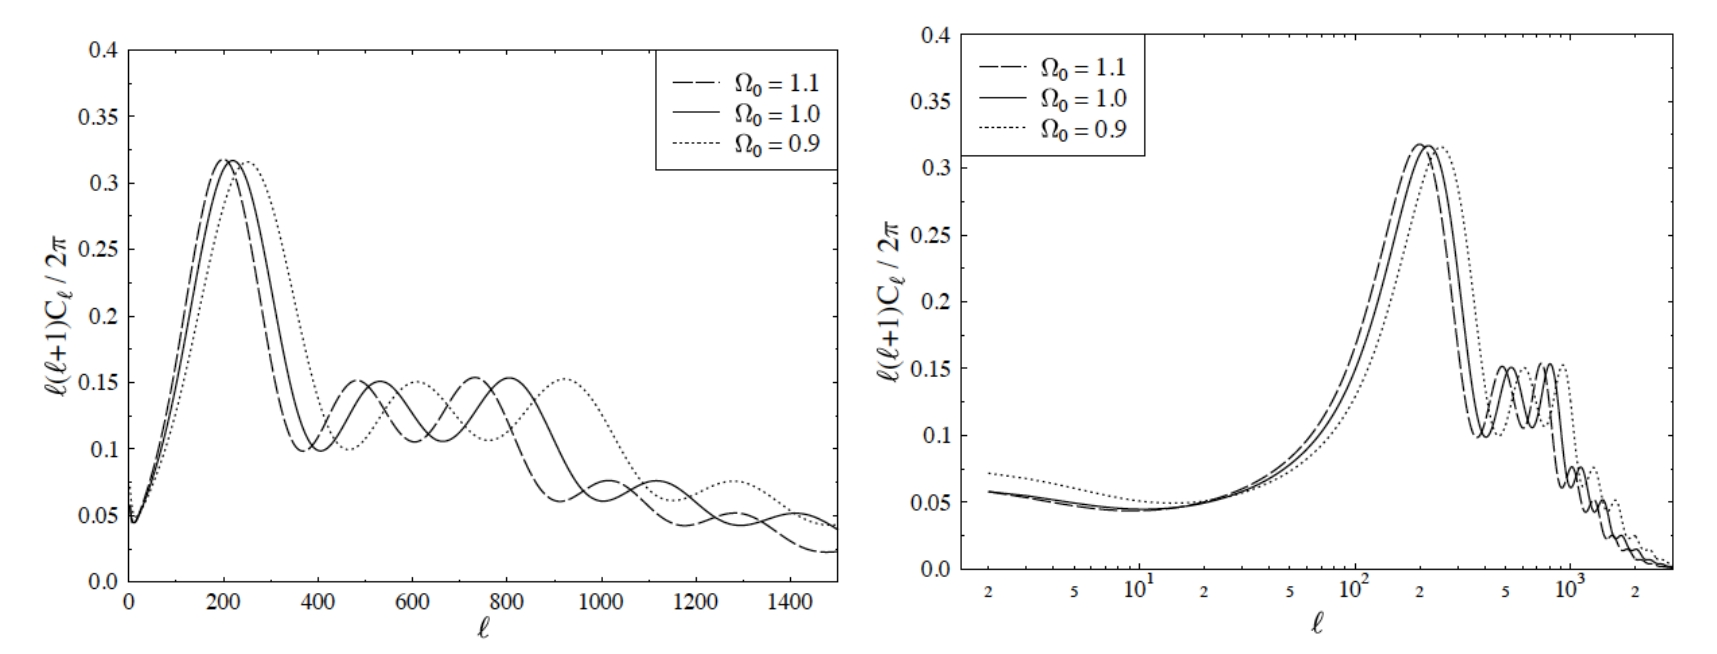
\includegraphics[width=0.9\textwidth]{images/omega_0_angular_power_spectrum.png}
    \caption{The effect of different values of $\Omega_0$ on the CMB power spectrum.}
    \label{fig:omega_0_angular_power_spectrum}
\end{figure}

%\clearpage
\bigskip \noindent
\begin{intuition}
    The above figure show the results of the CMB power spectrum for different values of $\Omega_0^{'}$ (the figure used $\Omega_0$ to represent $\Omega_0^{'}$ as different notations are used). \\
    
    With a fixed value of $\Omega_{\Lambda,0}$, we know the increasing value of $\Omega_0^{'}$ will cause a decrease of $d_A^c$, it make sense as it implies increasing of $\Omega_{m,0}$, which means more matter in the universe, and stronger deceleration of the expansion of the universe, and hence less distance and time that light can travel from the last-scattering surface to us. \\

    On the other hand, with a fixed value of $\Omega_{0}^{'}$, we know the increasing value of $\Omega_{\Lambda,0}$ will cause an increase of $d_A^c$, it also make sense as it implies more dark energy in the universe, which means stronger acceleration of the expansion of the universe, and hence more distance and time that light can travel from the last-scattering surface to us. \\

    Therefore, by measuring the positions of the acoustic peaks in the CMB power spectrum, we can infer important information about the curvature of the universe and the ratio of matter and dark energy in the universe. \\
\end{intuition}

\clearpage
%\bigskip \noindent
\begin{extra}
    you may wonder how we can measure the ratio of matter $\Omega_{m,0}$ and dark energy $\Omega_{\Lambda,0}$ and curvature $\Omega_{k,0}$ in the universe by just looking at the positions of the acoustic peaks in the CMB power spectrum, as there is 2 degree of freedom in the parameters, but we only have 1 degree of freedom in the positions of the acoustic peaks. \\

    The answer is we also measure other features in the CMB power spectrum, such as the relative heights of the acoustic peaks,  damping tail at small scales, and the Sachs-Wolfe effect at large scales, which can provide us more information about the universe, and help us to break the degeneracy between the parameters. We will discuss more about these features in next few sections.
\end{extra}

% -──────────────────────────────────────────────────────────────────────────────
\clearpage
%\bigskip \noindent \bigskip \noindent \bigskip \noindent
\subsection{Comoving Sound Horizon}
\begin{intuition}
    The comoving sound horizon $r_s(t_{rec})$ shows the comoving distance that a sound wave can travel from the beginning of the universe to the time of recombination. Note it is dependent on spacetime evolution \textbf{before} recombination.
\end{intuition}

\bigskip \noindent
\begin{foundation}
    The definition of the comoving sound horizon can be written as:
    \begin{align*}
        r_s^c(t_{rec}) &= \int_0^{t_{rec}} c_s^c(t) dt \\
        &= \int_0^{t_{rec}} \frac{c_s(t)}{a(t)} dt \\
        r_s^c(t_{rec}) &= \int_0^{a_{rec}} \frac{c_s(a)}{a^2 H(a)} da \\
        &= \int_0^{a_{rec}} \frac{c_s(a)}{a^2 H_0 \sqrt{\Omega_{m,0} a^{-3} + \Omega_{\Lambda,0} + \Omega_{k,0} a^{-2} + \Omega_{r,0} a^{-4}}} da \\
        &= \frac{1}{H_0} \int_0^{a_{rec}} \frac{c_s(a)}{\sqrt{\Omega_{m,0} a + \Omega_{\Lambda,0} a^4 + \Omega_{k,0} a^2 + \Omega_{r,0}}} da \\
            &= \frac{1}{H_0} \int_0^{a_{rec}} \frac{c_s(a)}{\sqrt{\Omega_{\Lambda,0} a^4 + (1 - \Omega_{0}^{'}) a^2 + \Omega_{m,0} a + \Omega_{r,0}}} da
    \end{align*}
    where $c_s(a)$ is the sound speed as a function of scale factor, and $H(a)$ is the Hubble parameter as a function of scale factor, and we used the definition of $\Omega_0^{'} = 1 - \Omega_{m,0} - \Omega_{\Lambda,0} - \Omega_{r,0}$ as the curvature density parameter. \\

    We can further take the assumption that in early stage of the universe $a \ll 1$, we can ignore the contribution of dark energy and curvature to the total energy density of the universe, and hence we can write $r_s^c(t_{rec})$ as:
    \begin{align*}
        r_s^c(t_{rec}) &= \frac{1}{H_0} \int_0^{a_{rec}} \frac{c_s(a)}{\sqrt{\Omega_{m,0} a + \Omega_{r,0}}} da
    \end{align*}
\end{foundation}

\clearpage
\begin{foundation}
    From the previous sections, we know the $c_s = \frac{1}{\sqrt{3}}$, but this is only true for the pure photon fluid, while in the real universe, we have baryons as well, which will affect the sound speed. The sound speed in the photon-baryon fluid can be expressed as:
    \begin{align*}
        c_s^2(a) &= \frac{\dot{P}}{\dot{\rho}} \\
        c_s^2(a) &= \frac{\dot{P}_\gamma + \dot{P}_b}{\dot{\rho}_\gamma + \dot{\rho}_b} \\
        c_s^2(a) &= \frac{\dot{P}_\gamma + 0}{\dot{\rho}_\gamma + \dot{\rho}_b} \\
        c_s^2(a) &= \frac{\dot{\rho}_\gamma / 3}{\dot{\rho}_\gamma + \dot{\rho}_b}
    \end{align*}

    Using the fluid continuity $\dot{\rho} = -3 H (\rho + P)$, we can get:
    \begin{align*}
        \begin{cases}
            \dot{\rho}_\gamma = -4 H \rho_\gamma \\
            \dot{\rho}_b = -3 H \rho_b
        \end{cases}
    \end{align*}
    Substituting the above equation back to the sound speed equation, we can get:
    \begin{align*}
        c_s^2(a) &= \frac{\dot{\rho}_\gamma / 3}{\dot{\rho}_\gamma + \dot{\rho}_b} \\
        c_s^2(a) &= \frac{\frac{-4 H \rho_\gamma}{3}}{-4 H \rho_\gamma - 3 H \rho_b} \\
        c_s^2(a) &= \frac{1}{3} \frac{4 \rho_\gamma}{4 \rho_\gamma + 3 \rho_b} \\
        c_s^2(a) &= \frac{1}{3} \frac{1}{1 + \frac{3 \rho_b}{4 \rho_\gamma}} \\
        c_s^2(a) &= \frac{1}{3} \frac{1}{1 + \frac{3}{4} \frac{\Omega_{b,0} a^{-3}}{\Omega_{\gamma,0} a^{-4}}} \\
        c_s^2(a) &= \frac{1}{3} \frac{1}{1 + \frac{3}{4} \frac{\Omega_{b,0}}{\Omega_{\gamma,0}} a}
    \end{align*}

    Therefore, we have the sound speed in the photon-baryon fluid as:
    \begin{align*}
        c_s^2(a) &= \begin{cases}
            \frac{1}{3} & \quad \text{, for pure photon fluid} \\
            \frac{1}{3} \frac{1}{1 + \frac{3}{4} \frac{\Omega_{b,0}}{\Omega_{\gamma,0}} a} & \quad \text{, for photon-baryon fluid}
        \end{cases}
    \end{align*}
\end{foundation}

%\clearpage
\begin{foundation}
    We can actually writing above equations in terms of physical density parameters $\omega_i = \Omega_{i,0} h^2$, where $h$ is the dimensionless Hubble parameter:
    \[
        h = \frac{H_0}{100\,\mathrm{km/s/Mpc}}
    \]
    and we can get:
    \begin{align*}
        c_s^2(a) &= \frac{1}{3} \frac{1}{1 + \frac{3}{4} \frac{\Omega_{b,0}}{\Omega_{\gamma,0}} a} \\
        c_s^2(a) &= \frac{1}{3} \frac{1}{1 + \frac{3}{4} \frac{\omega_b / h^2}{\omega_\gamma / h^2} a} \\
        c_s^2(a) &= \frac{1}{3} \frac{1}{1 + \frac{3}{4} \frac{\omega_b}{\omega_\gamma} a}
    \end{align*}
    substituting the above equation back to the $r_s^c(t_{rec})$ equation, we can get:
    \begin{align*}
        r_s^c(t_{rec}) &= \frac{1}{H_0} \int_0^{a_{rec}} \frac{c_s(a)}{\sqrt{\Omega_{m,0} a + \Omega_{r,0}}} da \\
        &= \frac{1}{100 h} \int_0^{a_{rec}} \frac{\frac{1}{\sqrt{3}} \frac{1}{\sqrt{1 + \frac{3}{4} \frac{\omega_b}{\omega_\gamma} a}}}{\sqrt{\omega_{m} \frac{a}{h^2} + \omega_{r} \frac{1}{h^2}}} da \\
        &= \frac{1}{100} \int_0^{a_{rec}} \frac{\frac{1}{\sqrt{3}} \frac{1}{\sqrt{1 + \frac{3}{4} \frac{\omega_b}{\omega_\gamma} a}}}{\sqrt{\omega_{m} a + \omega_{r}}} da \\
        &= \frac{1}{100} \int_0^{a_{rec}} \frac{1}{\sqrt{3}} \frac{1}{\sqrt{1 + \frac{3}{4} \frac{\omega_b}{\omega_\gamma} a}} \frac{1}{\sqrt{\omega_{m} a + \omega_{r}}} da \\
        &\approx 3000 \text{Mpc} \frac{1}{\sqrt{3 \omega_{r}}} \int_0^{a_{rec}} \frac{1}{\sqrt{1 + \frac{3}{4} \frac{\omega_b}{\omega_\gamma} a}} \frac{1}{\sqrt{1 + \frac{\omega_{m}}{\omega_{r}} a}} da
    \end{align*}
\end{foundation}

%\clearpage
\bigskip \noindent
\begin{theory}
    The comoving sound horizon at the time of recombination can be expressed as:
    \[
        r_s^c(t_{rec}) = r_s^c(\omega_b, \omega_d) =  \frac{3000 \text{Mpc}}{\sqrt{3 \omega_{r}}} \int_0^{a_{rec}} \frac{1}{\sqrt{1 + \frac{3}{4} \frac{\omega_b}{\omega_\gamma} a}} \frac{1}{\sqrt{1 + \frac{\omega_{m}}{\omega_{r}} a}} da
    \]
    where $\omega_b$ is the physical baryon density parameter, $\omega_\gamma$ is the physical photon density parameter ($ \approx 2.4702 \times 10^{-5}$ by CMB); $\omega_m$ is the physical matter density parameter, and $\omega_r$ is the physical radiation density parameter ($ \approx 4.1756 \times 10^{-5}$ by CMB).
\end{theory}

\bigskip \noindent
\begin{intuition}
    From the above equation, by given $\omega_\gamma$ and $\omega_r$ we can see that the roles of baryons and photons in the acoustic peaks; when $\omega_b$ increases, the baryon slow down the sound speed, it can be think as the more baryons in the photon-baryon fluid, the more inertia the fluid has, and hence the slower the sound speed. \\

    On the other hand, when $\omega_\gamma$ increases, the photons speed up the sound speed, it can be think as the more photons in the photon-baryon fluid, the more pressure the fluid has, and hence the faster the sound speed. \\

    Meanwhile, when $\omega_m$ increases, by Friedmann equation we can see that the expansion rate of the universe will increase, and hence the recombination time $t_{rec}$ happens earlier, hence a shorter time for the sound wave to travel, and hence a smaller sound horizon $r_s^c(t_{rec})$. And same for $\omega_r$ as well.
\end{intuition}

\clearpage
%\bigskip \noindent
\begin{example}{Numerical Estimate of the Acoustic Scale $l_A$}{acoustic-scale-estimate}
    Use representative values near recombination and Planck-like parameters:
    \[
        z_{rec}\approx 1090,
        \quad \Omega_{m,0}\approx 0.315,
        \quad \Omega_{\Lambda,0}\approx 0.685,
        \quad h\approx 0.674,
        \quad \omega_b\approx 0.0224.
    \]
    Break the estimate into three steps: \\
    (a). compute $d_A^c$; \\
    (b). compute $r_s^c$; \\
    (c). compute the acoustic peak scale.

    \bigskip\textbf{Solution.}\quad \\
    (a). \textbf{Comoving angular diameter distance} \\
    Use
    \[
        d_A^c(z_{rec}) = \int_0^{z_{rec}} \frac{dz}{H(z)},
        \qquad
        H(z)=H_0\sqrt{\Omega_{m,0}(1+z)^3+\Omega_{\Lambda,0}}
    \]
    (radiation gives only a small correction for this distance integral near late times). Numerically:
    \[
        d_A^c(z_{rec}) \approx 13.9\,\mathrm{Gpc} = 1.39\times 10^4\,\mathrm{Mpc}.
    \]

    (b). \textbf{Comoving sound horizon} \\
    Use
    \[
        r_s^c(t_{rec}) = \int_0^{a_{rec}} \frac{c_s(a)}{a^2 H(a)}\,da,
        \qquad
        c_s(a)=\frac{1}{\sqrt{3\left(1+\frac{3}{4}\frac{\omega_b}{\omega_\gamma}a\right)}}.
    \]
    Numerically (with the above Planck-like parameters):
    \[
        r_s^c(t_{rec}) \approx 144\,\mathrm{Mpc}.
    \]

    (c). \textbf{Acoustic peak scale} \\
    First compute
    \[
        \theta_s = \frac{r_s^c}{d_A^c}
        \approx \frac{144}{1.39\times 10^4}
        \approx 1.04\times 10^{-2}\,\mathrm{rad}
        \approx 0.60^\circ.
    \]
    Then
    \[
        l_A = \frac{\pi}{\theta_s}
        = \pi\frac{d_A^c}{r_s^c}
        \approx \frac{3.1416}{1.04\times10^{-2}}
        \approx 302 \approx 300.
    \]
    Therefore, the fundamental acoustic spacing scale is $l_A\sim 300$, while the first temperature peak is observed near $l\sim 220$ due to phase-shift/projection effects.
\end{example}



% =══════════════════════════════════════════════════════════════════════════════
\clearpage
%\bigskip \noindent \bigskip \noindent \bigskip \noindent
\section{More Features of the Power Spectrum}
From the previous section, we have discussed about the acoustic peaks in the power spectrum, which is the most prominent feature in the power spectrum. However, you may noticed we have ignored the damping term in the equation of temperature perturbation, which is not our real case. In fact, during the oscillation of the photon-baryon fluid, the oscillation is not perfect, but is damped by the expansion of the universe and the diffusion of photons (Silk damping). Therefore, we need to consider the damping term in the equation of temperature perturbation, which will give us more features in the power spectrum, such as the damping tail at small scales. \\

Besides, there are also other features in the power spectrum, such as the Sachs-Wolfe effect at large scales, and the relative heights of the acoustic peaks, which can provide us more information about the universe, such as the geometry of the universe, we will discuss more about these features in below subsections.

% -──────────────────────────────────────────────────────────────────────────────
\bigskip \noindent \bigskip \noindent %\bigskip \noindent
\subsection{Damping Tail}
\begin{intuition}
    If we further consider the damping term, we can write the oscillation equation of the photon-baryon fluid as:
    \[
        \ddot{\Theta} + c_s^2 k^2 f(c_i) \Theta + c_s^2 k^2 \Theta = g(c_i)
    \]
    where $f(c_i)$ is the damping term by the expansion of the universe and the diffusion of photons, and $g(c_i)$ is the source term by the gravitational potential. The $c_i$ are the parameters that affect the damping and source terms, such as the baryon density, the matter density, the dark matter density, etc. \\

    We can simply write the damping coeffcient as:
    \[
        c \propto k^2 \propto l^2
    \]
    Therefore, for the small scales (large $l$), the damping term will be more significant, and hence the amplitude of the oscillation will be smaller, which will give us a damping tail in the power spectrum at small scales.
\end{intuition}

\bigskip \noindent
\begin{foundation}
    To connect the above oscillator picture with the observed power spectrum, we can separate damping into two intuitive effects:
    \begin{itemize}
        \item \textbf{Expansion damping (Hubble friction):} the expansion of the universe removes energy from oscillations, similar to friction in a damped oscillator.
        \item \textbf{Diffusion damping (Silk damping):} before decoupling, photons still scatter many times and perform a random walk, so they can leak from hot regions to cold regions and smooth out temperature contrast.
    \end{itemize}

    The second effect is the dominant reason for the sharp small-scale suppression. A useful way to state it is: modes with wavelength smaller than the photon diffusion scale are exponentially erased. In $k$-space, this is often written schematically as:
    \[
        \Theta(k,\eta_*) \simeq \Theta_{\mathrm{osc}}(k,\eta_*)\,\exp\!\left[-\left(\frac{k}{k_D}\right)^2\right]
    \]
    where $k_D$ is the diffusion-damping scale (evaluated near recombination), and $\eta_*$ is recombination time. \newline

    Since larger $k$ means smaller physical scale, the exponential factor suppresses high-$k$ modes much more strongly. This is exactly the same trend as your earlier statement $c\propto k^2\propto l^2$: higher-$k$ (thus higher-$l$) modes damp faster.
\end{foundation}

\bigskip \noindent
\begin{theory}
    A compact way to summarize the damping-tail physics is:
    \[
        \Theta(k)\;\text{is multiplied by}\;\exp\!\left[-\left(\frac{k}{k_D}\right)^2\right]
        \quad\Longrightarrow\quad
        C_l\;\text{is suppressed at large }l.
    \]

    Using the projection relation $l\sim k\,d_A^c$ (with $d_A^c$ the comoving angular-diameter distance to last scattering), we define a damping multipole $l_D\sim k_D d_A^c$. Then the observed spectrum is often approximated by:
    \[
        C_l \simeq C_l^{\mathrm{(no\ damping)}}\,\exp\!\left[-2\left(\frac{l}{l_D}\right)^2\right]
    \]
    up to order-one modeling details.

    Therefore, the high-$l$ side of the CMB spectrum is not another acoustic peak sequence, but a progressively damped tail: the smaller the angular scale, the stronger the suppression by photon diffusion (plus expansion damping).
\end{theory}

\begin{figure}[!htbp]
    \centering
    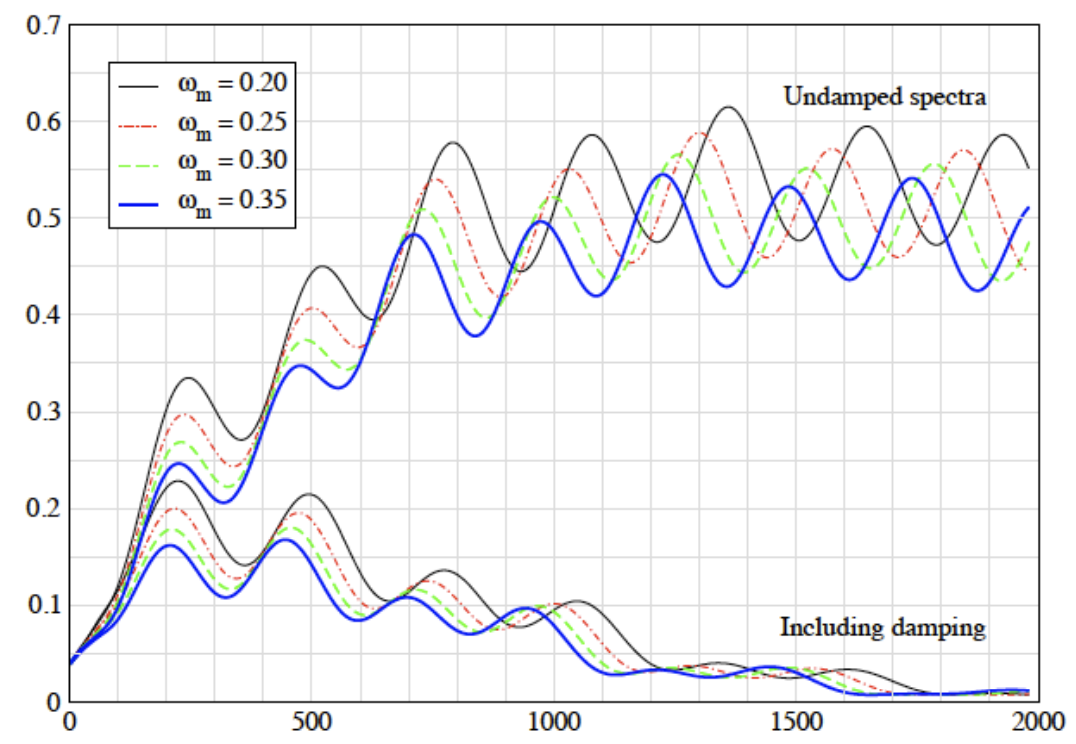
\includegraphics[width=0.9\textwidth]{images/damping_tail.png}
    \caption{The effect of damping on the CMB power spectrum.}
    \label{fig:damping_tail}
\end{figure}


% -──────────────────────────────────────────────────────────────────────────────
\bigskip \noindent \bigskip \noindent \bigskip \noindent
\subsection{Sachs-Wolfe Effect}
\begin{intuition}
    The Sachs-Wolfe (SW) effect describes how gravity changes the observed CMB temperature when photons travel from the last-scattering surface to us. \\

    A simple picture is: imagine photons are emitted from different ``gravitational landscapes'' (potential wells and hills). If a photon climbs out from a potential well, it loses energy (gravitational redshift), so we observe it colder; if it is emitted from a potential hill, it gains relative energy and looks hotter. This converts gravitational potential perturbations directly into temperature anisotropies. \\

    There are two related contributions:
    \begin{itemize}
        \item \textbf{Ordinary Sachs-Wolfe (OSW):} set at recombination, mainly important on very large angular scales.
        \item \textbf{Integrated Sachs-Wolfe (ISW):} accumulated during photon propagation when gravitational potentials evolve with time.
    \end{itemize}
    Therefore, the SW effect is the key physical reason why the low-$l$ (large-angle) part of the CMB power spectrum carries direct information about primordial metric perturbations and late-time expansion history.
\end{intuition}

\bigskip \noindent
\begin{foundation}
    Let the line-of-sight direction be $\hat{n}$ and conformal time be $\eta$. The observed temperature perturbation can be written schematically as:
    \[
        \Theta(\hat{n}) \equiv \frac{\Delta T}{T_0}(\hat{n})
        = \left[\Theta_0 + \Psi\right]_{*}
        + \int_{\eta_*}^{\eta_0} \left(\dot{\Psi} + \dot{\Phi}\right) d\eta
    \]
    where:
    \begin{itemize}
        \item $\Theta_0$ is the intrinsic photon temperature perturbation at last scattering;
        \item $\Psi$ and $\Phi$ are metric (gravitational potential) perturbations;
        \item subscript $*$ means evaluated at recombination;
        \item the integral term is along the photon path from recombination to today.
    \end{itemize}

    The first bracket term is the \textbf{ordinary SW} contribution, while the line-of-sight integral is the \textbf{ISW} contribution. \\

    For super-horizon modes at recombination in matter domination (and negligible anisotropic stress, so $\Phi \simeq \Psi$), the ordinary SW term reduces to the well-known approximation:
    \[
        \left(\frac{\Delta T}{T_0}\right)_{\mathrm{OSW}} \simeq \frac{1}{3}\Psi_*
    \]
    (up to sign convention of the potential). \\

    Physically, this means large-angle CMB anisotropy is roughly one-third of the primordial gravitational potential perturbation at last scattering. \\

    For the ISW term:
    \begin{itemize}
        \item During strict matter domination, potentials are nearly constant, so $\dot{\Psi}+\dot{\Phi}\approx 0$, and ISW is small.
        \item Near radiation-matter transition (early ISW) and in dark-energy domination (late ISW), potentials evolve, so ISW becomes non-zero.
    \end{itemize}
\end{foundation}

\bigskip \noindent
\begin{theory}
    The Sachs-Wolfe contribution to CMB anisotropy can be summarized as:
    \[
        \Theta(\hat{n})
        = \underbrace{\left[\Theta_0 + \Psi\right]_*}_{\text{ordinary SW}}
        + \underbrace{\int_{\eta_*}^{\eta_0} (\dot{\Psi}+\dot{\Phi}) d\eta}_{\text{integrated SW}}
    \]
    and for large scales at recombination:
    \[
        \left(\frac{\Delta T}{T_0}\right)_{\mathrm{OSW}} \simeq \frac{1}{3}\Psi_*
    \]

    In the angular power spectrum, this physics appears as the low-$l$ Sachs-Wolfe plateau (roughly $l \lesssim 30$), where:
    \[
        \frac{l(l+1)C_l}{2\pi} \approx \text{constant}
    \]
    while late-time ISW slightly modifies the largest scales and provides sensitivity to dark energy and spatial curvature.
\end{theory}

% -──────────────────────────────────────────────────────────────────────────────
\bigskip \noindent \bigskip \noindent \bigskip \noindent
\subsection{Relative Heights of the Acoustic Peaks}
\begin{intuition}
    To understand why different peaks have different heights, we only need three physical ideas that we already introduced in previous sections: \textbf{compression vs rarefaction}, \textbf{baryon inertia}, and \textbf{gravitational potential wells}. \\

    Before recombination, each Fourier mode of the photon-baryon fluid oscillates like a driven oscillator. At decoupling, we take a ``snapshot'' of all modes:
    \begin{itemize}
        \item modes caught at \textbf{maximum compression} (odd peaks: 1st, 3rd, 5th, ...) produce one set of peak heights;
        \item modes caught at \textbf{maximum rarefaction} (even peaks: 2nd, 4th, ...) produce another set.
    \end{itemize}

    If we add more baryons, the fluid has more mass (inertia). This shifts the oscillation zero-point toward compression, so compressions become deeper while rarefactions become shallower. Therefore, increasing baryon density enhances \textbf{odd peaks relative to even peaks}. \\

    Dark matter contributes mainly through gravity: it deepens potential wells and changes how strongly modes are driven around horizon entry. This affects the overall peak envelope and, in particular, the height of higher peaks (for example the third peak) relative to lower ones. \\

    So the pattern of peak heights is not random: odd-even contrast mainly traces baryons, while the broader peak-height pattern across multiple peaks is sensitive to total matter and dark matter.
\end{intuition}

\bigskip \noindent
\begin{foundation}
    A useful approximate form of the photon temperature perturbation for one mode is:
    \[
        \Theta_0(k,\eta_*) + \Psi(k,\eta_*)
        \approx A(k) \cos\!\big(k\,r_s(\eta_*)\big) - R_*\,\Psi(k,\eta_*)
    \]
    where:
    \begin{itemize}
        \item $r_s(\eta_*)$ is the sound horizon at recombination;
        \item $R_* \equiv \frac{3\rho_b}{4\rho_\gamma}\big|_{*}$ measures baryon loading;
        \item $A(k)$ encodes driving effects from the evolving gravitational potentials.
    \end{itemize}

    The cosine term gives the alternating compression/rarefaction phases, while the $-R_*\Psi$ term is the baryon-loading shift. As $R_*$ increases:
    \begin{itemize}
        \item compression extrema (odd peaks) are boosted;
        \item rarefaction extrema (even peaks) are suppressed.
    \end{itemize}

    Meanwhile, matter content controls potential evolution around horizon entry:
    \begin{itemize}
        \item more matter (especially non-baryonic dark matter) makes potentials decay less during the radiation-to-matter transition;
        \item this changes the driving efficiency and therefore the relative heights among the first few peaks, especially the third peak compared with the first two.
    \end{itemize}
\end{foundation}

\bigskip \noindent
\begin{theory}
    The relative peak heights provide complementary parameter sensitivity:
    \begin{align*}
        \text{odd/even contrast} &\longrightarrow \omega_b \;(=\Omega_{b,0}h^2), \\
        \text{higher-peak pattern (e.g. 3rd vs 1st/2nd)} &\longrightarrow \omega_m \;(=\Omega_{m,0}h^2), \\
        \text{with }\omega_m-\omega_b &\text{ isolating dark matter density }\omega_c.
    \end{align*}

    In practice, CMB fits use the full spectrum shape, but an intuitive summary is:
    \begin{itemize}
        \item larger $\omega_b$ $\Rightarrow$ stronger odd peaks relative to even peaks;
        \item larger $\omega_c$ (or total $\omega_m$ at fixed $\omega_b$) $\Rightarrow$ modified driving and a characteristic change in the third and higher peaks.
    \end{itemize}

    Therefore, combining peak positions (geometry) with peak heights (dynamics) lets us separately constrain baryons, dark matter, and total matter in the standard cosmological model.
\end{theory}

% =══════════════════════════════════════════════════════════════════════════════
\clearpage
%\bigskip \noindent \bigskip \noindent \bigskip \noindent
\section{CMB and $\Lambda$CDM-Standard Model}
\begin{extra}
    %\small
    The discovery of the Cosmic Microwave Background (CMB) in 1964 provided decisive evidence for the Hot Big Bang model, but the composition and energy budget of the universe remained uncertain for decades. \\

    In the 1970s, cosmological models were often constrained to baryonic matter alone, motivated by Occam's razor and early estimates of the cosmic density. However, these pure-baryon models faced severe theoretical and observational tensions. First, Big Bang Nucleosynthesis (BBN) strictly limited the baryon density to $\Omega_b \lesssim 0.05$, far below the critical density suggested by inflation. Second, because baryons were tightly coupled to photons until recombination ($z \sim 1100$), radiation pressure suppressed gravitational collapse, making it impossible to form the observed large-scale structure within the age of the universe. Additionally, early estimates of the Hubble constant implied a universe younger than the oldest globular clusters, creating the age problem. \\

    In the 1980s, the Cold Dark Matter (CDM) paradigm emerged, proposing that the universe is dominated by non-baryonic, weakly interacting particles that decoupled from radiation early on. Because CDM is unaffected by photon pressure, its density perturbations could begin growing immediately after inflation, providing the gravitational scaffolding for baryonic structure formation. While CDM successfully resolved the structure formation problem, a flat, matter-dominated universe still required a low Hubble constant ($H_0 \lesssim 50$ km/s/Mpc) to match stellar ages, which increasingly conflicted with direct distance-ladder measurements. \\

    In the 1990s, two major extensions were explored: the mixed Hot+Cold Dark Matter (HCDM) model and the $\Lambda$CDM model. The 1992 COBE detection of CMB anisotropies, combined with large-scale structure surveys, began to favor models with a cosmological constant $\Lambda$. The discovery of cosmic acceleration in 1998 via Type Ia supernovae provided direct evidence for $\Lambda$ (or dark energy), which naturally resolved the age problem by altering the expansion history and increasing the cosmic age for a given $H_0$. By the late 1990s and early 2000s, $\Lambda$CDM emerged as the consensus model, consistently fitting CMB power spectra, baryon acoustic oscillations, supernova distances, and the growth of structure, eventually becoming the standard model of cosmology.
    %\normalsize
\end{extra}

% \clearpage
% \begin{figure}
%     \centering
%     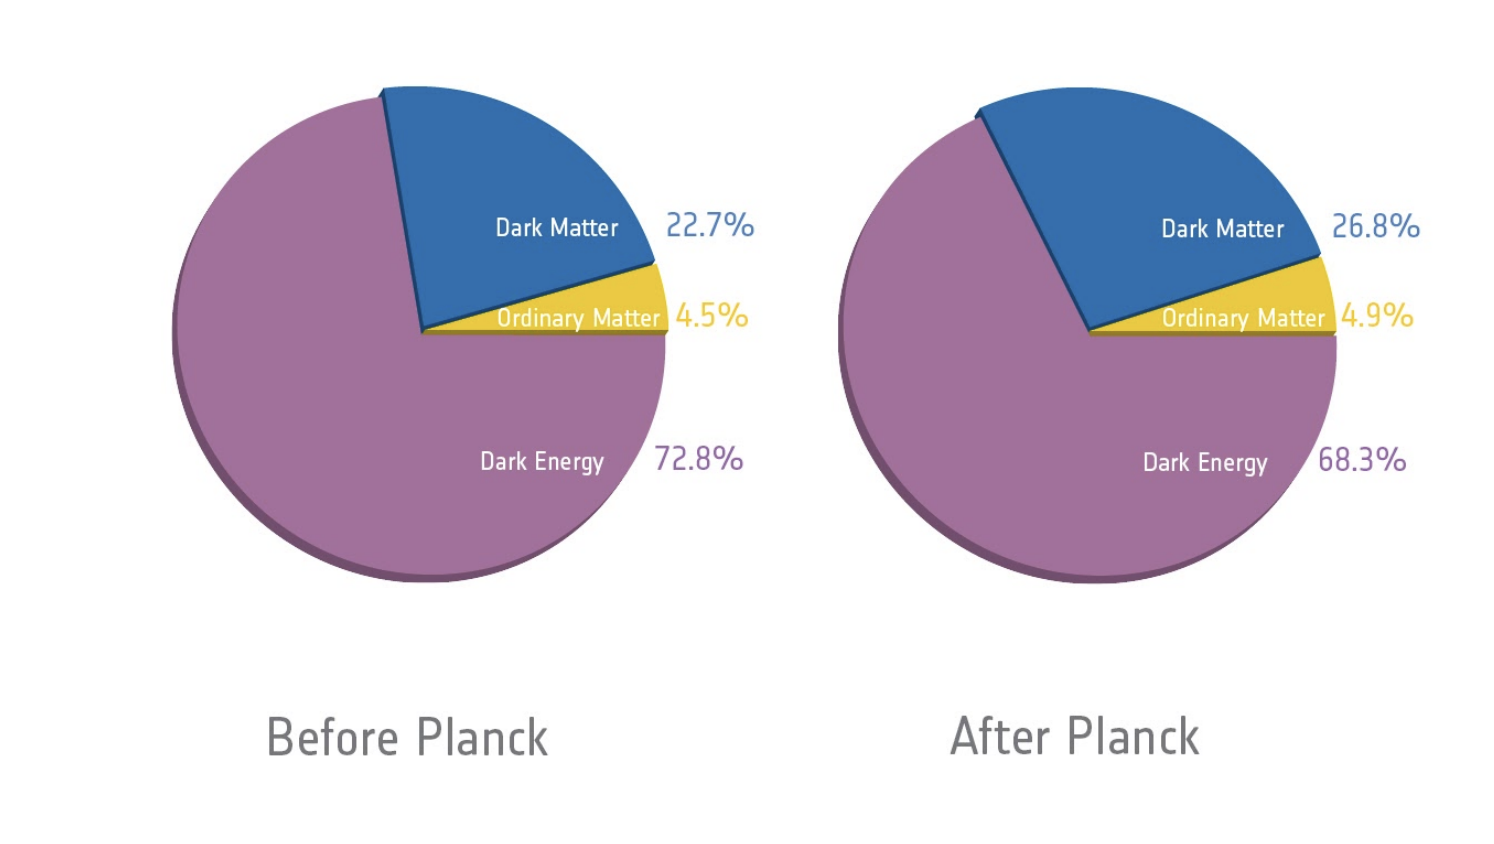
\includegraphics[width=0.9\textwidth]{images/cosmic_recipe.png}
%     \caption{The cosmic recipe before(left) and after(right) the Planck 2018 results.}
%     \label{fig:cosmic_recipe}
% \end{figure}